\pdfoutput=1
\documentclass[cits]{JINST}
\newcommand{\unit}[1]{\ensuremath{\mathrm{\,#1}}}
\renewcommand{\u}[1]{\unit{#1}}
\newcommand{\um}{\textmu m}
\DeclareFontFamily{U}{euc}{}
\DeclareFontShape{U}{euc}{m}{n}{<-6>eurm5<6-8>eurm7<8->eurm10}{}
\DeclareSymbolFont{AMSc}{U}{euc}{m}{n}
\DeclareMathSymbol{\umu}{\mathord}{AMSc}{"16}
\usepackage[justification=centering]{caption}
\usepackage[pdftex]{graphicx}
\usepackage{amsmath}
\usepackage{afterpage}
\usepackage{wrapfig}
\usepackage{tabularx}
\usepackage{subfigure}
\usepackage{caption}
\usepackage{tabu}
\usepackage{booktabs}
\usepackage{multicol}
\newcommand{\comment}[1]{{\fontsize{10}{10}{\par \tt\textbf {\selectfont #1}} \par}}

\graphicspath{{figs/}}

\usepackage{lineno}
\linenumbers

\title{Separation of nearby hadronic showers in the CALICE SDHCAL prototype detector using ArborPFA}

\author{R. \'Et\'e$^a$\thanks{Corresponding author.} \\%, I. Laktineh$^a$ , G. Grenier$^a$ , A. Steen$^a$ , L. Mirabito$^a$\\
\llap{$^a$} Universit\'e de Lyon, Universit\'e Lyon 1, CNRS/IN2P3, 
 IPNL, 4 Rue E.~Fermi, 69622 Villeurbanne Cedex, France\\
 
 
 E-mail: \email{rete@ipnl.in2p3.fr}
 }
 
\abstract
{
A new reconstruction algorithm, ArborPFA, is developed to separate nearby hadronic showers in the SDHCAL prototype. This intends to demonstrate the capability of high granularity hadronic calorimeters such as the SDHCAL to efficiently apply Particle Flow Algorithms. The reconstruction algorithm we present here uses the tree-like structure features of hadronic showers, that high granular calorimeters reveal, to associate hits belonging to each hadronic shower and to reduce confusions between two close-by showers. The results of these studies indicate a good single particle efficiency and reconstructed energy. A powerful separation down to distance of 5 cm was also pointed out.
}

\begin{document}

\keywords{Keywords: Particle flow; Calorimetry; ILC; SDHCAL}

\newpage
\section{Introduction}
%%%%%%%%%%%%%%%%%%%%%%%%%%%%%%%%%%%%%%%%%%%
%%%%%%%%%%%%%%%%%%%%%%%%%%%%%%%%%%%%%%%%%%%

~~~~~~~To study the Higgs boson properties and to extend the discovery of new particles beyond the scope of LHC, linear (e.g ILC) and circular (e.g FCC or CEPC) e$^+$ e$^-$ colliders are proposed. An important requirement of such a machine is to provide a good jet energy resolution ($\Delta$E/E $\sim$3-4\%) in order to distinguish between Z and W$^{\pm}$ bosons as well as to study the Higgs boson properties.

The Particle Flow concept has been proposed to achieve the ILC benchmarks \cite{ilc-tdr}. This algorithm aims to individually reconstruct particles using the most appropriate sub-detector for the energy and momentum measurement. An implementation of the particle flow algorithm called PandoraPFA has been developed \cite{pandora-pfa} and successfully applied in ILD physics performance studies and to close-by hadronic showers separation%\cite{note ahcal !!!}.

To apply efficiently the Particle Flow Algorithms, both good energy resolution and fine transverse and longitudinal segmentation should be provided by the \textit{electromagnetic calorimeter} (ECAL) and the \textit{hadronic calorimeter} (HCAL).

Different calorimeter technologies are currently under study by the CALICE collaboration to fulfill these requirements. In this framework, a \textit{semi digital hadronic calorimeter} prototype (SDHCAL) was built \cite{sdhcal-paper} and successfully tested at the CERN H6 test beam lines of the SPS (CERN) in 2012. With a transverse readout segmentation of 1 cm$^2$, 48 sampling layers and good energy resolution \cite{sdhcal-paper}, this calorimeter statifies ILC requirements. 

In this paper, we present an other approach of the particle flow : the ArborPFA approach. The algorithm has been designed for high granularity calorimeters and applied to SDHCAL test beam data. We propose to evaluate the performance of the algorithm on single pion events and to study the ability of the algorithm to separate two overlaid pion showers at different separation distances and energies.

\newpage
\section{The SDHCAL prototype}

The SDHCAL prototype is a sampling calorimeter which consists of 48 layers alternating a 20 mm steel absorbers and a 6 mm gas resistive plate chamber (GRPC) with their embedded electronics. The gas gap between the two electrodes of the GRPC is 1.2 mm. 9216 pads (96 x 96) of 1cm$^2$ compose the readout of each chamber, leading to a total number of 442368 channels. Signals from particles crossing the gas gap are recorded on those pads in a 2-bits format corresponding to 3 thresholds on the induced charge. A complete description of the calorimeter setup and its features can be found in \cite{sdhcal-paper}. 

The test beam data used in this paper were taken at the CERN H6 beam line in 2012. The pion event selection is also performed according to the selection presented in \cite{sdhcal-paper}.

The reconstructed energy of a single particle is computed as follows :

\begin{equation}
  E_{rec} = \alpha(N_{hit}) \cdot N_{1}
          + \beta(N_{hit}) \cdot N_{2}
          + \gamma(N_{hit}) \cdot N_{3}   
\end{equation}
where N$_1$, N$_2$ and N$_3$ are the number hits of threshold 1, 2 and 3, N$_{hit}$ = N$_1$ + N$_2$ + N$_3$ and $\alpha$, $\beta$ and $\gamma$ are quadratic functions of the number of hits N$_{hit}$. The nine parameters of these functions are extracted from a $\chi^2$ minimization :

\begin{equation}
  \chi^2 = \sum\limits_{evt} \frac{(E_{beam} - E_{rec})^2}{E_{beam}}
\end{equation}
This minimization was performed over all the hadronic events in the energy range [10, 80] GeV by step of 10 GeV. No weight is assigned event by event either per energy point. The linearity and energy resolution will be shown in section \ref{SINGLE_PARTICLE_STUDY_SECTION} dedicated to the single particle study.

\newpage
\section{The Arbor particle flow algorithm}
%%%%%%%%%%%%%%%%%%%%%%%%%%%%%%%%%%%%%%%%%%%
%%%%%%%%%%%%%%%%%%%%%%%%%%%%%%%%%%%%%%%%%%%

~~~~~~~The Arbor approach has been developed by the ALEPH collaboration and recently adapted \cite{arbor-manqi} for ILD detector design. It is based on the idea that the hadronic shower development follows a tree-like topology.

Figure \ref{ARBOR_STRUCTURE} shows an example of a shower development (left) where all main components of the shower are present : charged particles, neutral particles, electromagnetic and hadronic components.
The same figure shows on the right a sampling calorimeter view of a shower interaction as seen in a highly granular calorimeter. The black arrows drawn on this view suggest the tree-like topology development of the shower.

With such an approach, the shower reconstruction follows a principle close to the underlying physics.

\begin{figure}[!ht]
  \begin{center}
    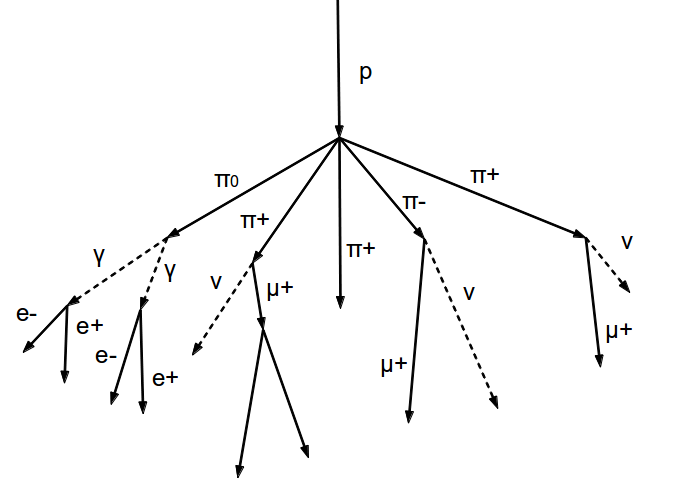
\includegraphics[width=0.45\linewidth]{ProtonDecay.png} \hfill
    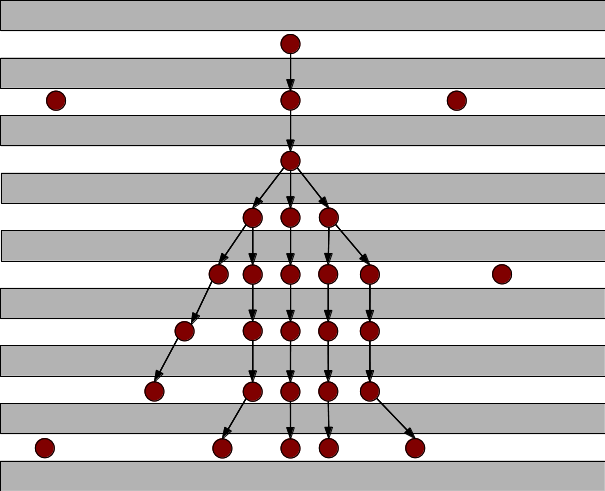
\includegraphics[width=0.45\linewidth]{ArborSchema.png}
  \end{center}
  \caption{\label{ARBOR_STRUCTURE} Left : schematic view of an induced proton shower. Right : schematic view of a reconstructed shower in a calorimeter with calorimeter hits (red)}
\end{figure}

The algorithm we used here is implemented using the PandoraSDK API as a toolkit for generic PFA development \cite{pandora-sdk}. The API is used in a Marlin \cite{marlin-lccd} C++ processor as part of the reconstruction chain in ILCSOFT \cite{ilcsoft}. A complete description of the algorithm can be found in Appendix \ref{ARBOR_ALGO_DESCRIPTION}

%%%%%%%%%%%%%%%%%%%%%%%%%%%%%%%%%%%
%%%%%% Single particle study %%%%%%
%%%%%%%%%%%%%%%%%%%%%%%%%%%%%%%%%%%
\newpage
\section{Single particle study}
\label{SINGLE_PARTICLE_STUDY_SECTION}

\subsection{Setup}

\begin{wrapfigure}{r}{0.45\textwidth}
  \vspace{-20pt}
  \begin{center}
    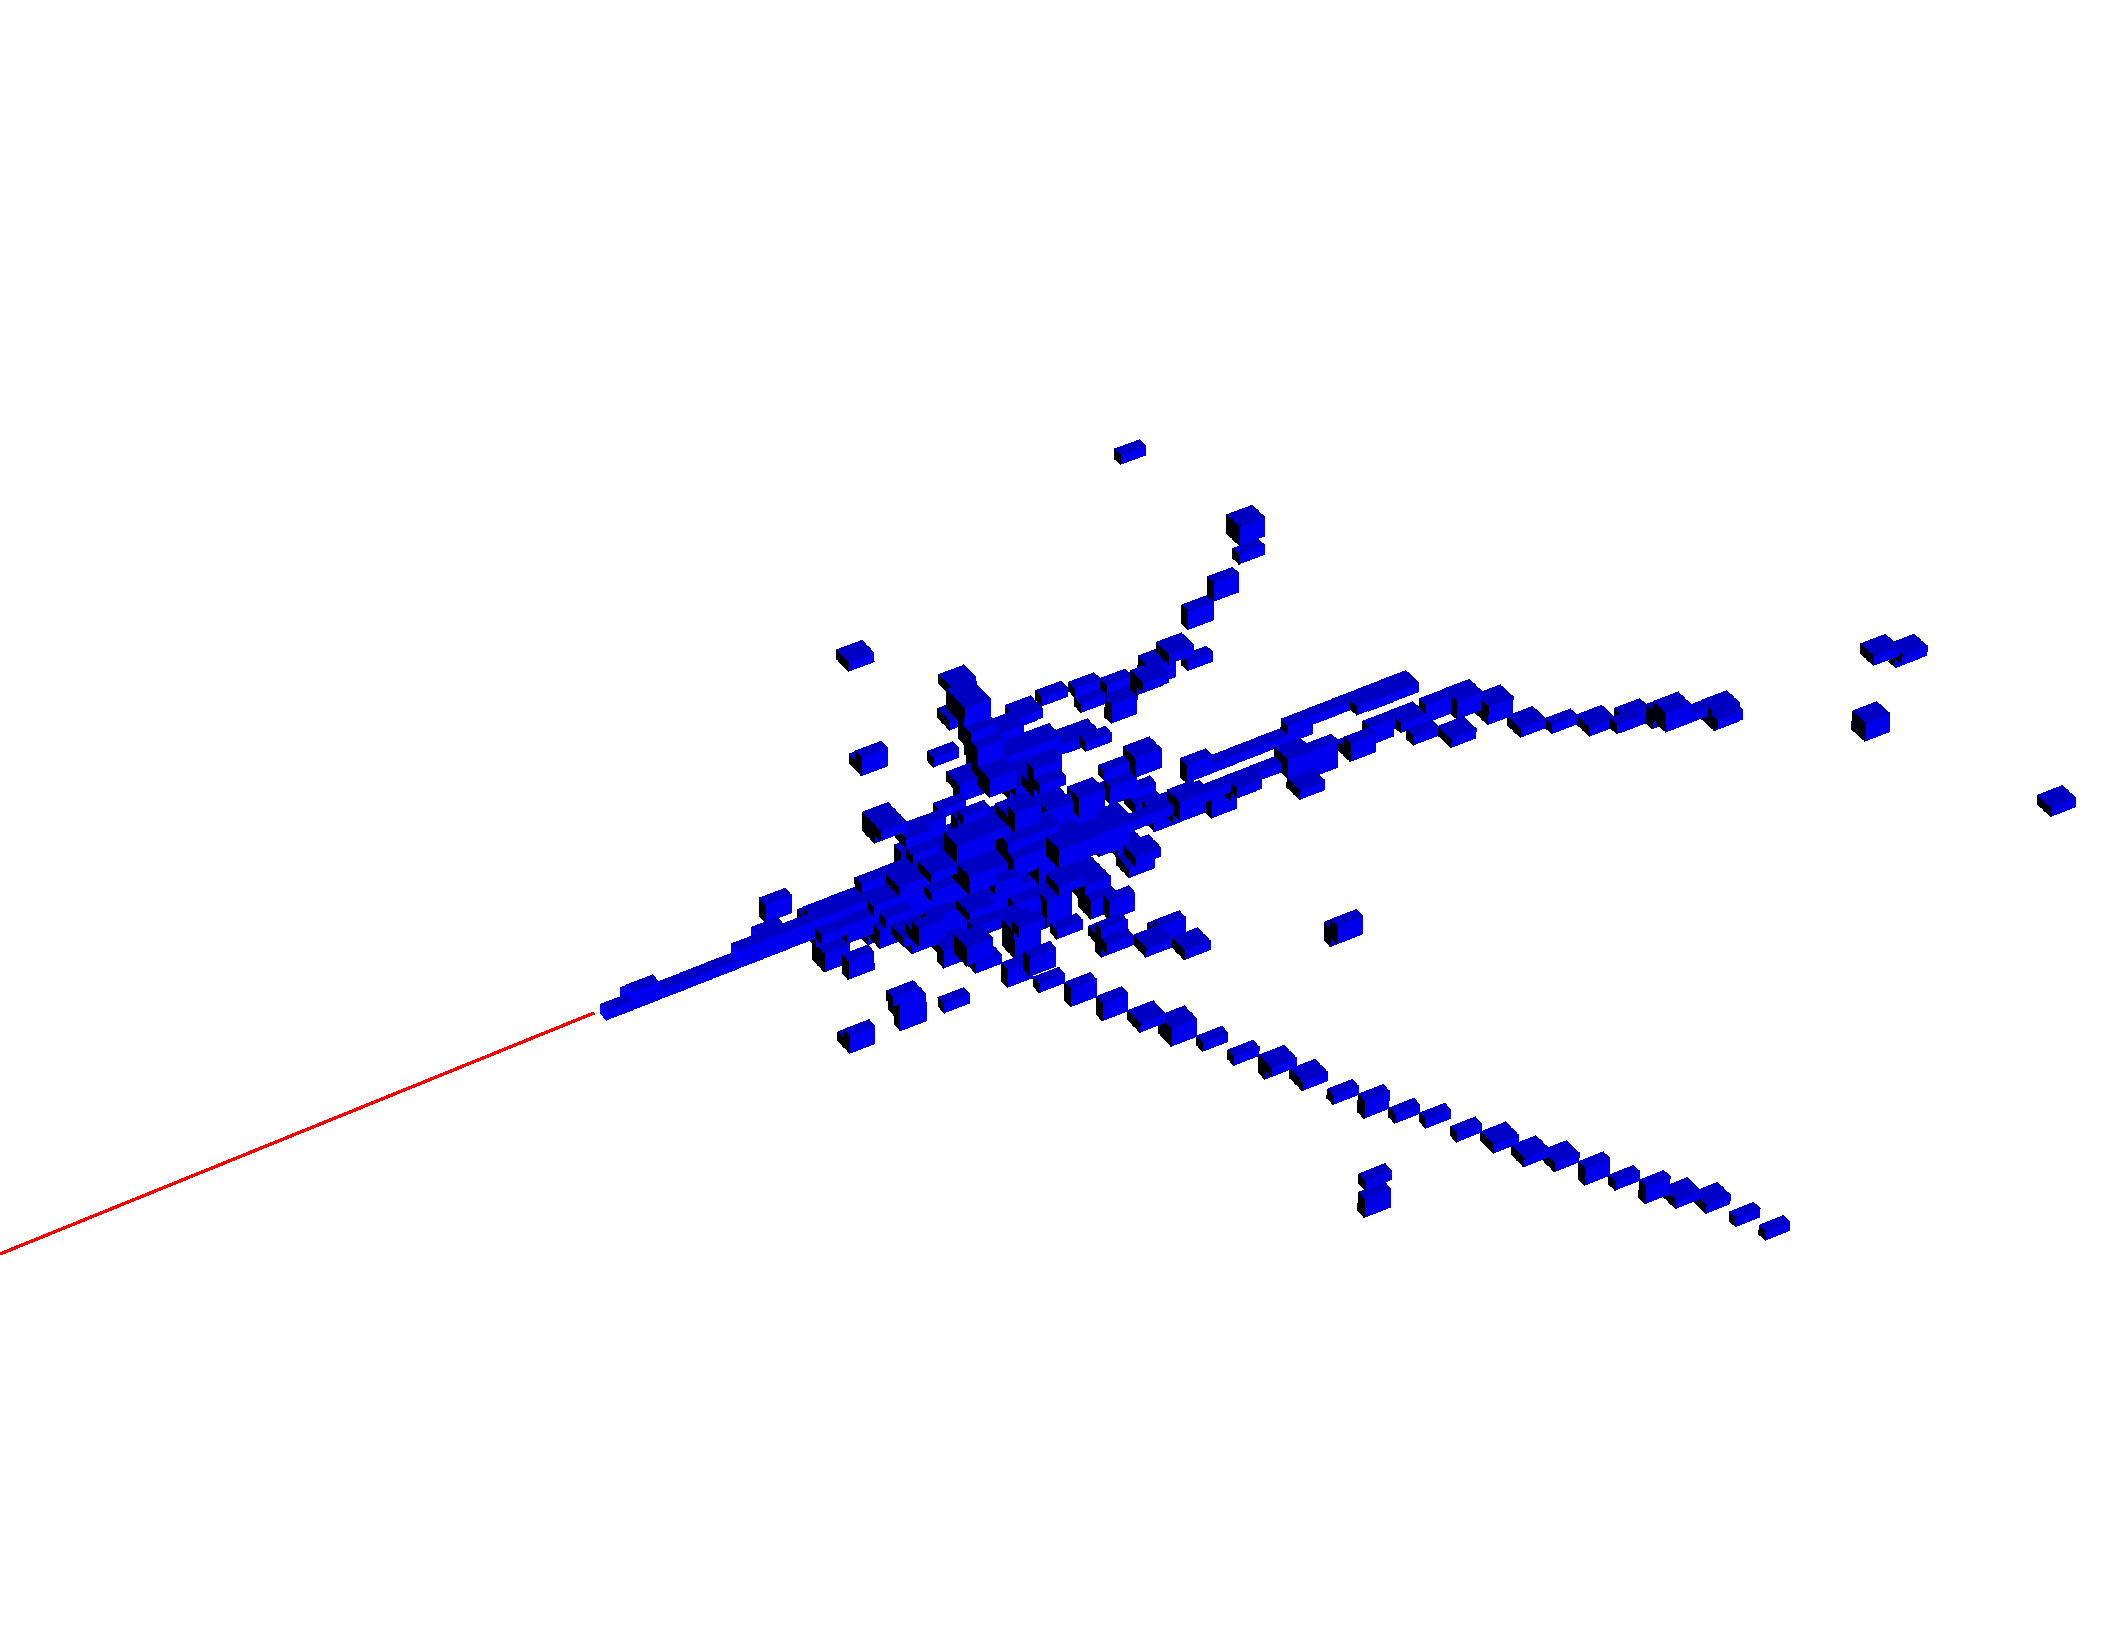
\includegraphics[width=\linewidth]{SingleParticleSetup.pdf}
  \end{center}
  \vspace{-10pt}
  \caption{\label{ARBOR_SINGLE_PARTICLE_SETUP} Event display of a 50 GeV pion shower in the SDHCAL detector}
\end{wrapfigure}

To study the single particle performance of the algorithm, we use the SDHCAL charged pion data taken at CERN on the H6 line of SPS in 2012 from 10 GeV up to 80 GeV. In order to select only pions, an event selection is performed as described in \cite{sdhcal-paper}.

To correctly emulate a charged pion for the reconstruction program and since there was no tracker in front of the SDHCAL during beam tests, a fake track is created in front of the calorimeter. A global barycentre of all hit positions in the transverse plane (X and Y axes) is calculated. A new barycentre is then calculated using only hits n the 4 first layers and within a region of 8x8 cells around the global barycentre in the X and Y directions. This defines the shower entering point in the first layer. From the entering point of the shower, a straight track is created along the beam axis (Z direction) with momentum equal to that of beams.

The calorimeter hits and the created track are then loaded into the PandoraSDK toolkit \cite{pandora-sdk} within a single hcal endcap geometry (no magnetic field) with the SDHCAL prototype dimensions and processed by the ArborPFA algorithms. An event display of a single pion event is shown on figure~\ref{ARBOR_SINGLE_PARTICLE_SETUP}.

\subsection{Single particle analysis}

\begin{figure}[!h]
  \begin{center}
    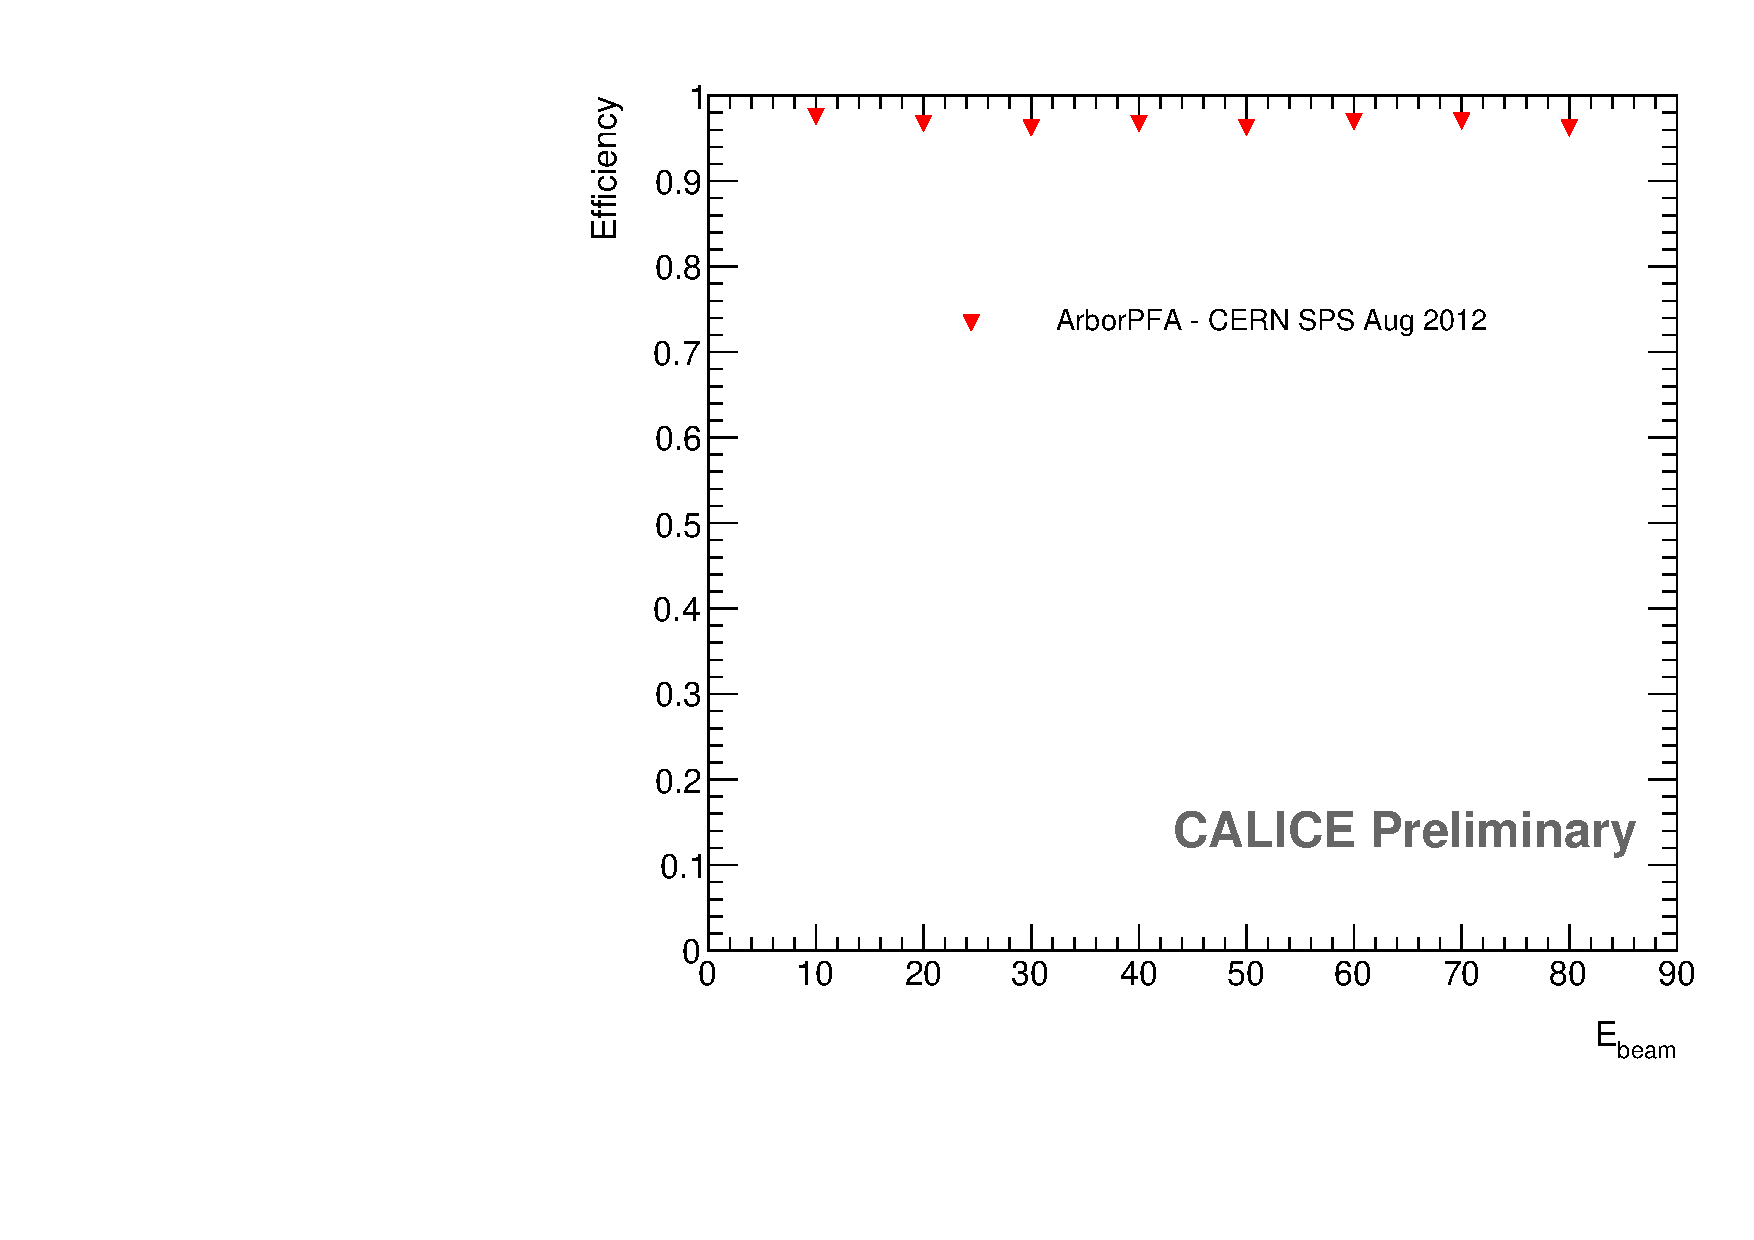
\includegraphics[width=0.48\textwidth]{plots/SingleParticle_Efficiency.pdf}
    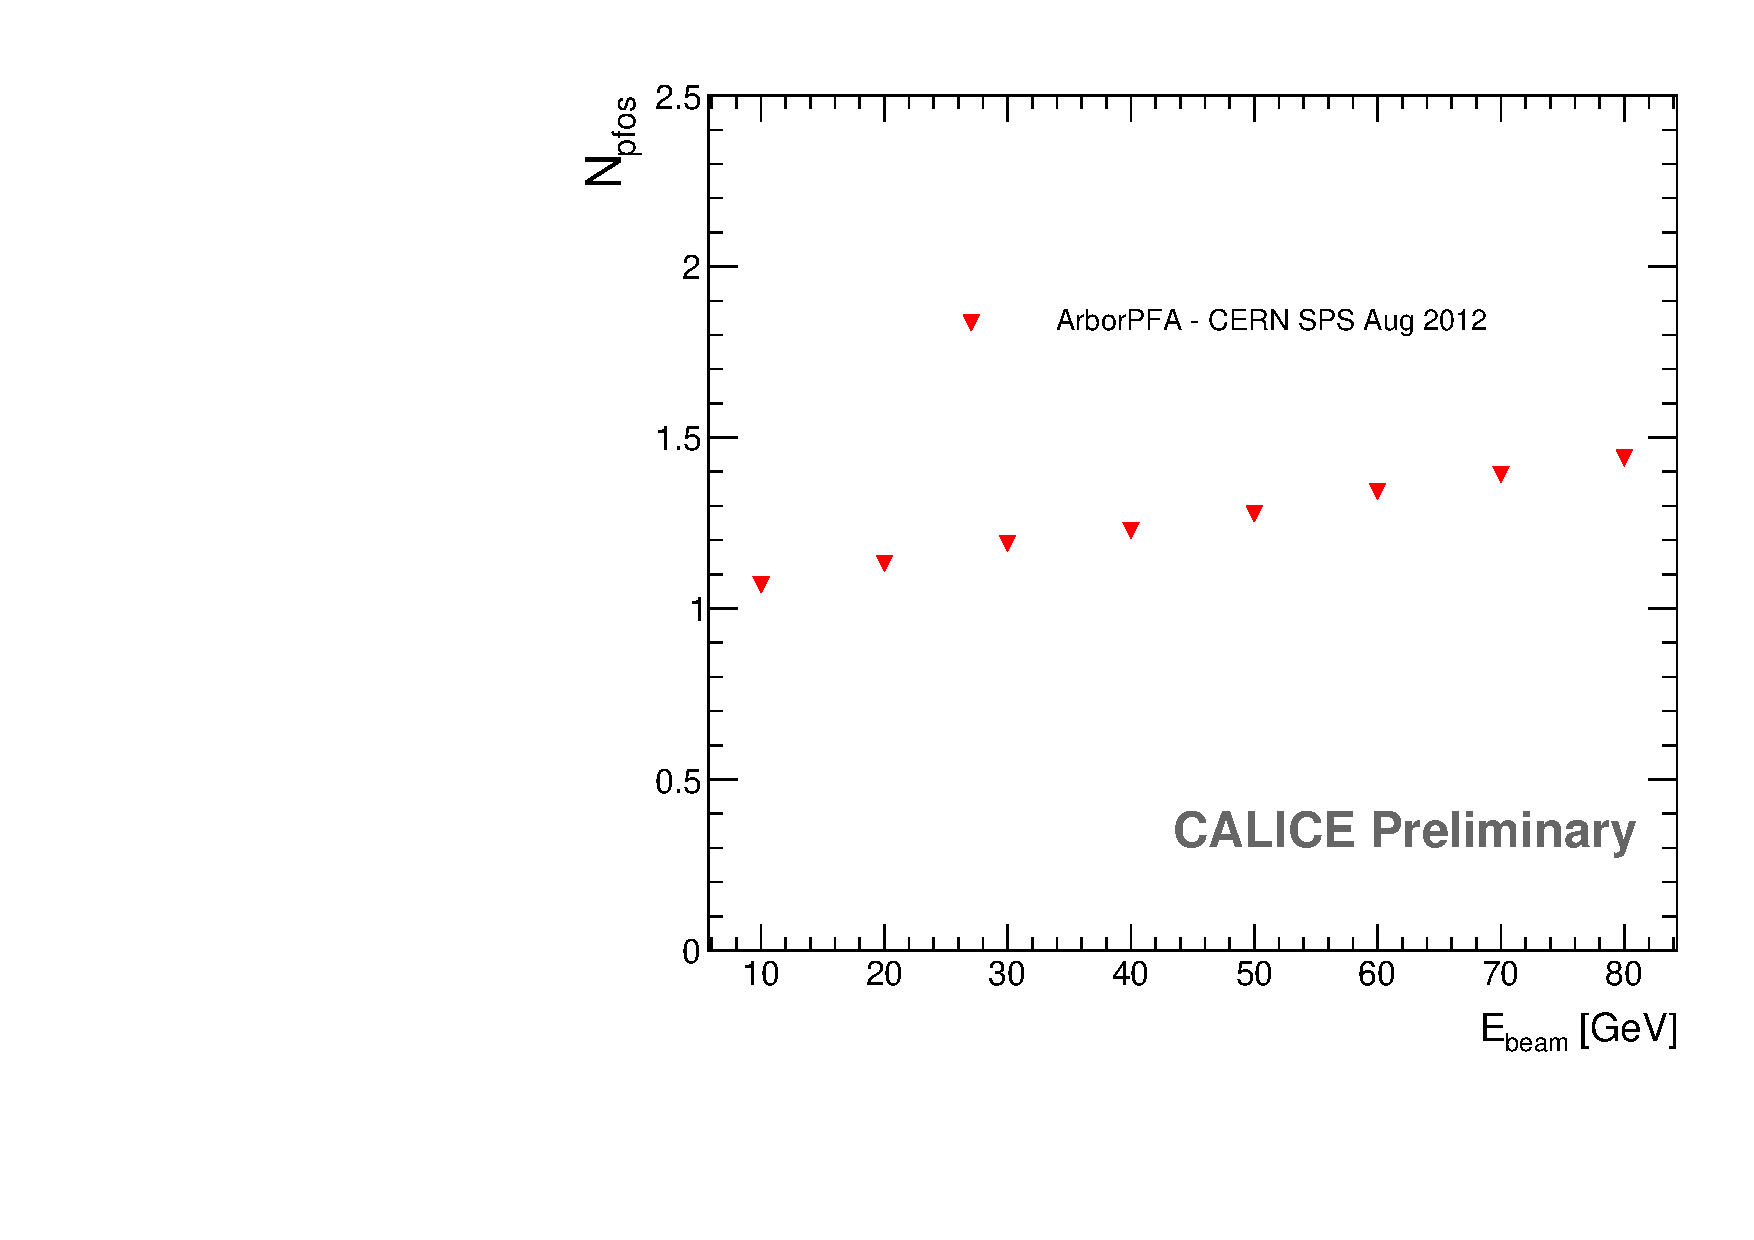
\includegraphics[width=0.48\textwidth]{plots/SingleParticle_NPfos.pdf} \\
  \end{center}
  \caption{\label{ARBOR_SINGLE_PARTICLE_EFFICIENCY_AND_NPFOS} Hit clustering efficiency (left) and the mean number of reconstructed particles (right) after ArborPFA reconstruction on single pion shower events with the SDHCAL prototype}
\end{figure}

We define the efficiency of the single particle reconstruction, or the hit clustering efficiency $\epsilon_s$ as the fraction of hits recovered by the ArborPFA program and correctly attached to track in front of the calorimeter. Figure \ref{ARBOR_SINGLE_PARTICLE_EFFICIENCY_AND_NPFOS} shows the mean efficiency of the single particle reconstruction (left) and the mean number of reconstructed particles (right) as a function of the beam energy after applying ArborPFA. It shows a constant efficiency of over 96\% over the whole beam energy range. Since the number of hits increases with the energy, the number of missed hits in the reconstructed charged particle also increases. Consequently, the mean number of reconstructed particles shows an increase which is directly due to shower splitting. This number grows up to 1.45 particles at 80 GeV but has only a small impact on the reconstructed energy and energy resolution because the small additional clusters represent a small amount of energy. Indeed, figure \ref{ARBOR_SINGLE_PARTICLE_EREC_AND_ERESOL} shows the reconstructed energy and energy resolution of a single charged pion before and after running the ArborPFA program. 

\begin{figure}[!h]
  \begin{center}
    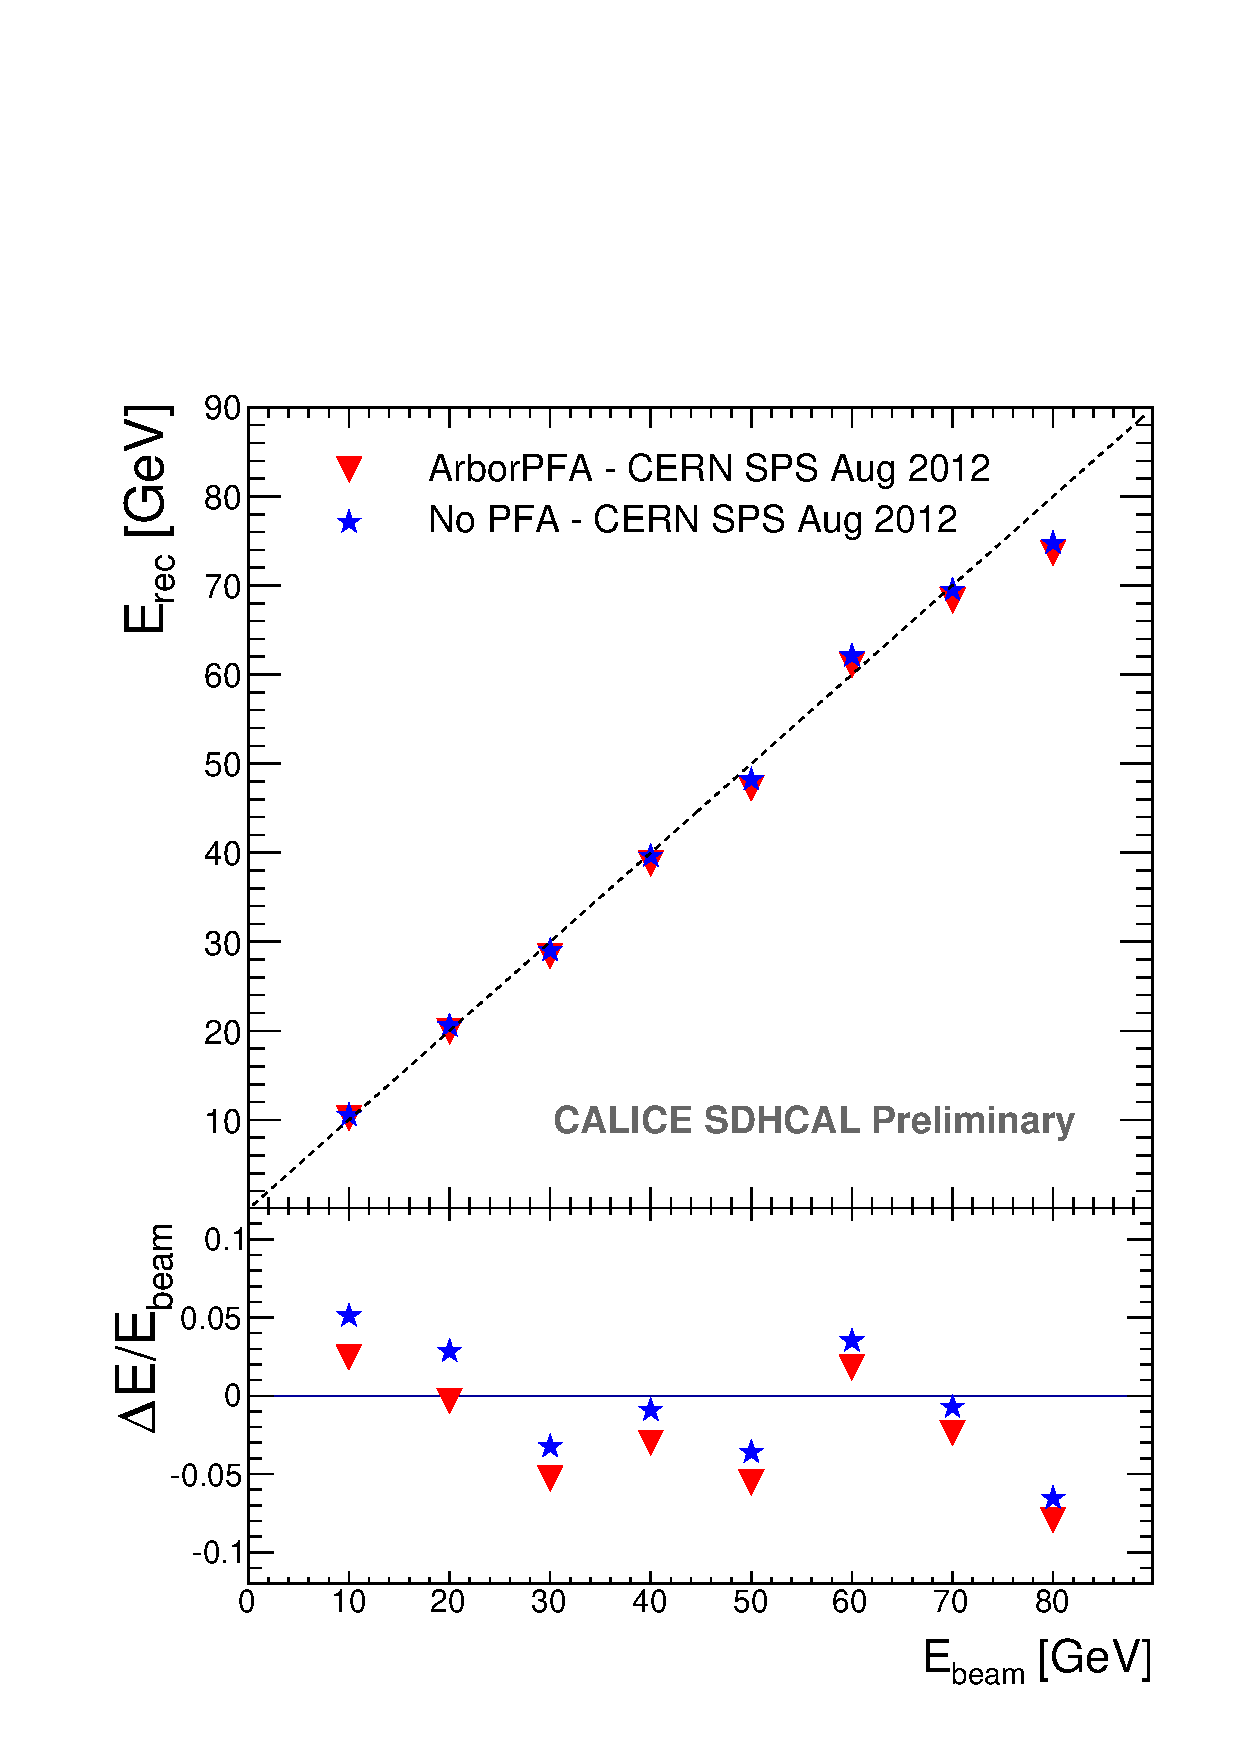
\includegraphics[width=0.48\textwidth]{plots/SingleParticle_ERec.pdf}
    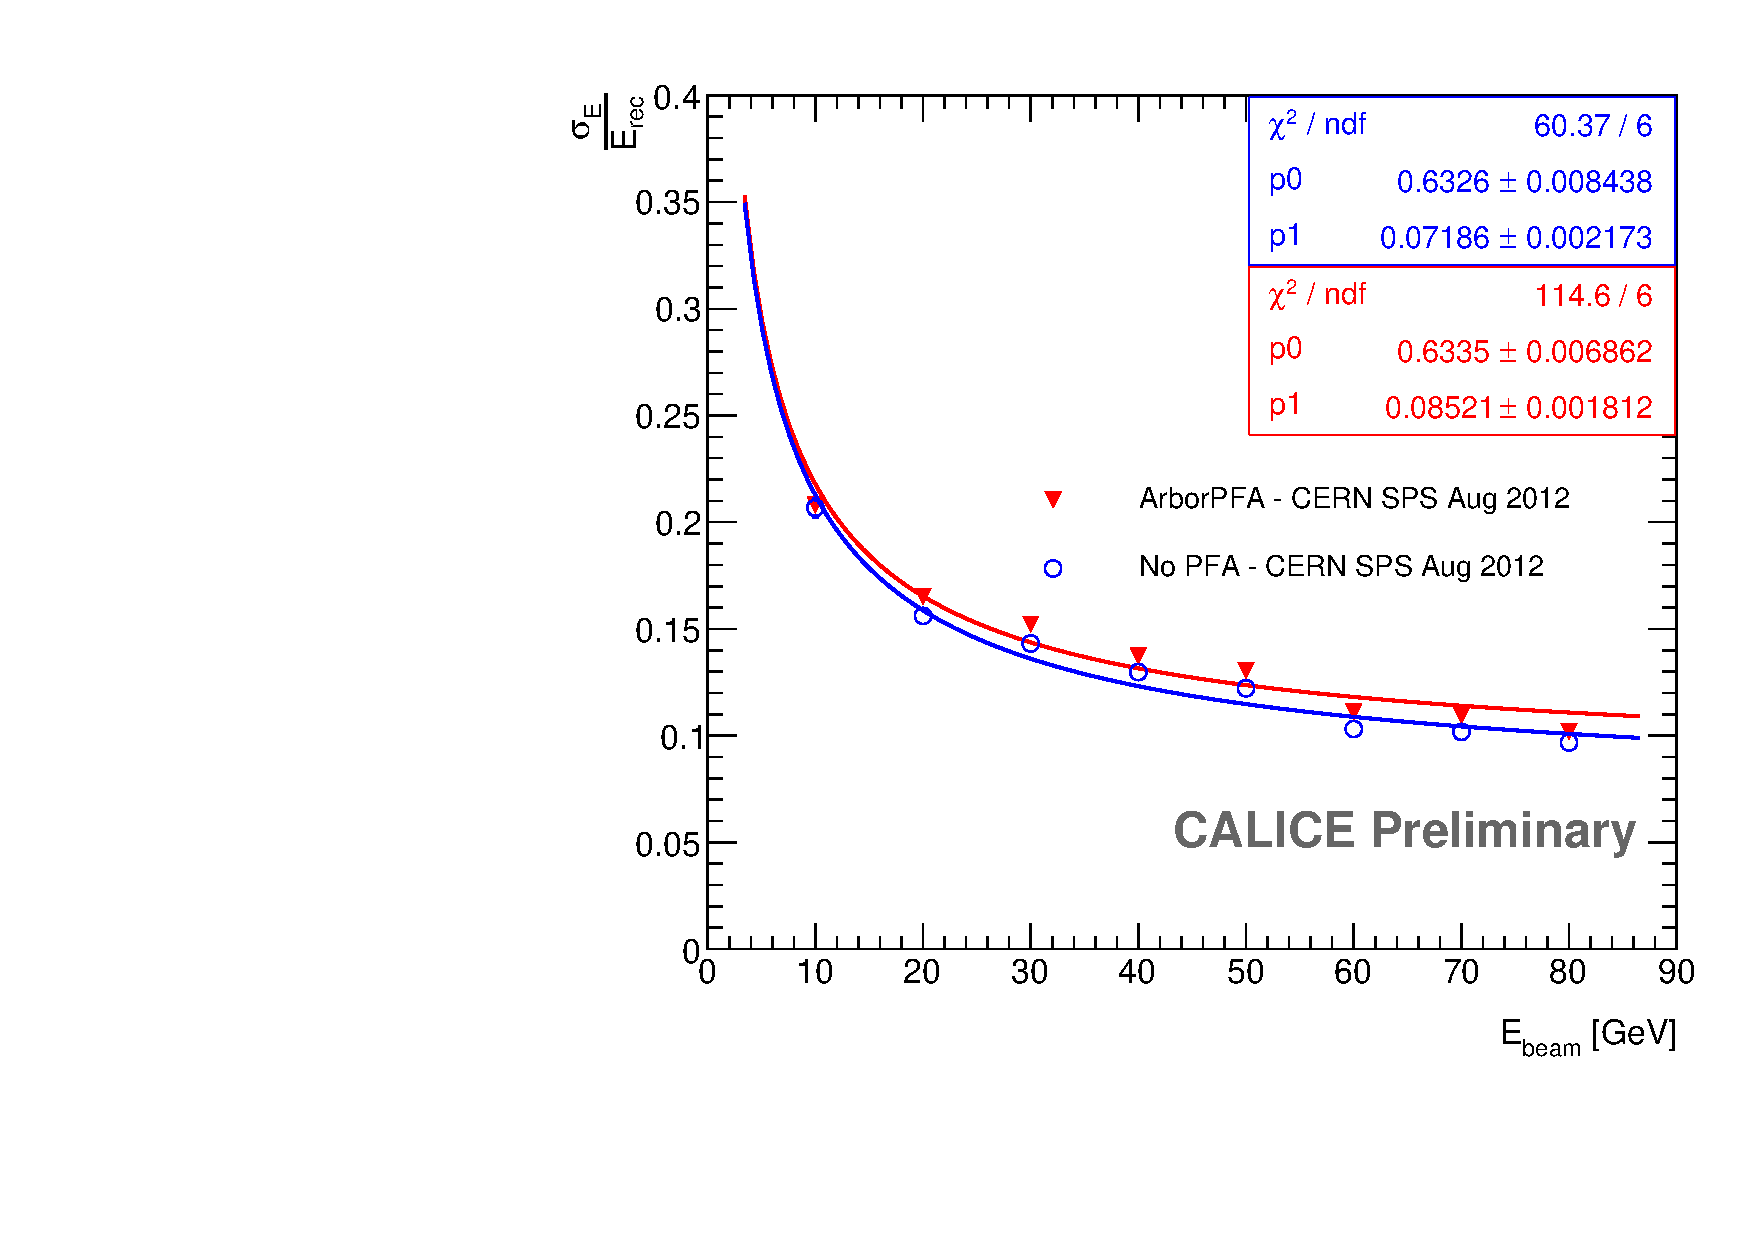
\includegraphics[width=0.48\textwidth]{plots/SingleParticle_EResol.pdf} \\
  \end{center}
  \caption{\label{ARBOR_SINGLE_PARTICLE_EREC_AND_ERESOL} Reconstructed energy (left) and energy resolution (right) before (blue) and after (red) ArborPFA reconstruction on single pion shower event with the SDHCAL prototype}
\end{figure}

The deviation from linearity is shown below the reconstructed energy and is defined as :

\begin{equation}
  \Delta E/E_{beam} = \Big(E_{rec} - E_{beam}\Big)/E_{beam}
\end{equation}

These energy points are extracted using two fits of the energy distributions : i) a gaussian distribution fit over the full reconstructed distribution is first performed. The mean $\mu_{E,first}$ and width $\sigma_{E,first}$ are extracted, and ii) a second gaussian fit is then performed over the range [$\mu_{E,first}$-1.5*$\sigma_{E,first}$ ; $\mu_{E,first}$+1.5*$\sigma_{E,first}$]. From the latter, we extract the final values of the reconstructed energy and energy resolution defined as the mean $\mu_E$ and the width $\sigma_E$ respectively of the gaussian fit (same procedure applied in \cite{sdhcal-paper}). The efficiency plot has shown that some hits are missing after reconstruction so it is expected to have a small energy decrease in the reconstructed energy. Nevertheless, the linearity is still within 8\% as before applying the reconstruction. The energy resolution is also not so much affected after reconstruction.

%%%%%%%%%%%%%%%%%%%%%%%%%%%%%%%%%%%%%%%%%%%%%%%%%%%%%
%%%%%% Separation of two close-by hadronic showers %%%%%%
%%%%%%%%%%%%%%%%%%%%%%%%%%%%%%%%%%%%%%%%%%%%%%%%%%%%%
\newpage
\section{Separation of two close-by hadronic showers}

The ability of a particle flow algorithm to disentangle close-by showers is a key point for the reconstruction in detectors such as ILD of the ILC. To study the confusion between neutral and charged hadrons and the ability of the ArborPFA algorithm to disentangle them, we again use the same test beam data of the SDHCAL prototype. Two different pion showers are first overlaid in the same event and the ArborPFA algorithm is run on the overlaid event with the same parameters as for the single particle study. An analysis of the separation is then performed in order to extract the performance of the algorithm.

\subsection{Overlay procedure and setup}

In order to study the separation of nearby hadronic showers, two events from test beam data are overlaid in one event. We have chosen to overlay 10 GeV pion events and pion events at different energies from 10 GeV to 50 GeV, in steps of 10 GeV. The distance between shower entry points was scanned between 5 cm and 30 cm in steps of 5 cm. The choice of this energy range is motivated by the fact that it is the typical single particle energies foreseen at the ILC within jets \cite{hadron-jets}.

\begin{figure}[!h]
  \begin{center}
    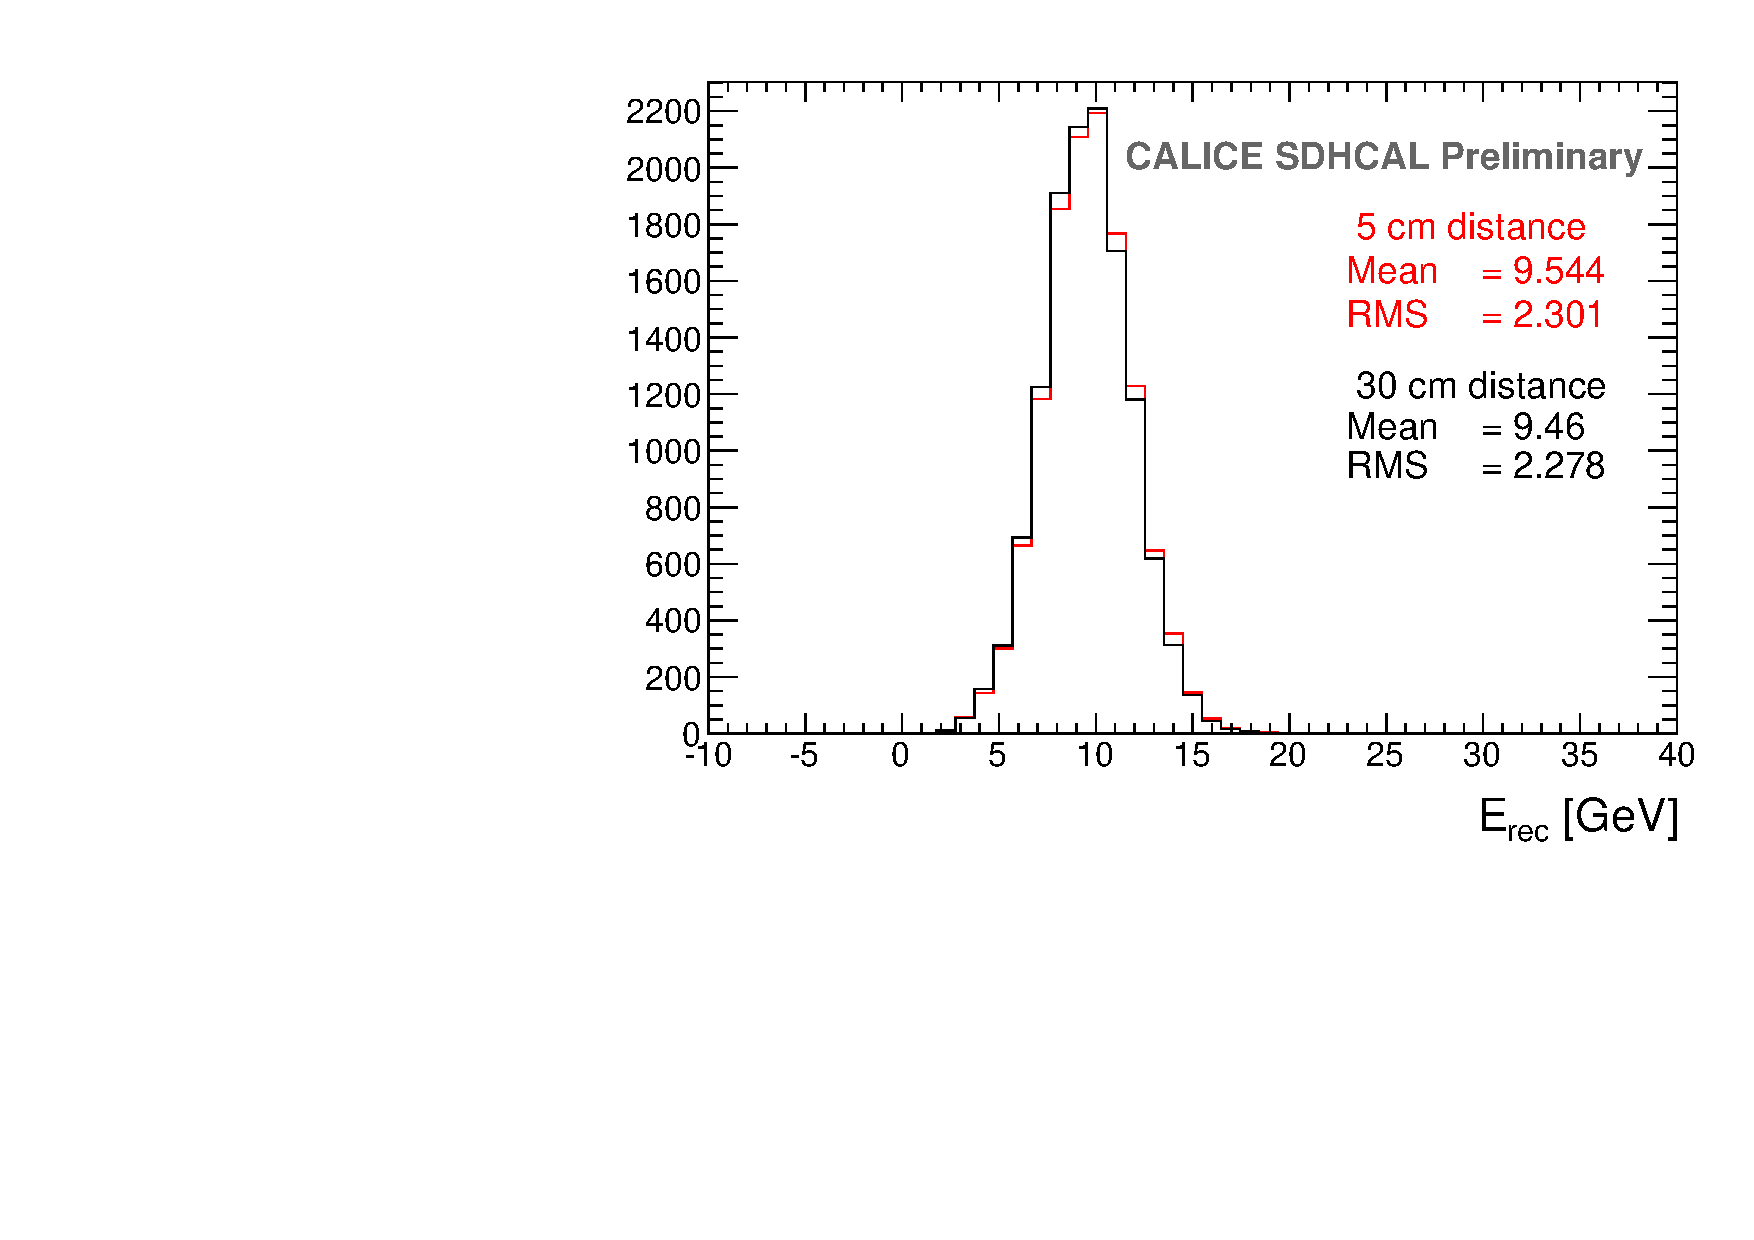
\includegraphics[width=0.6\linewidth]{plots/OverlayEvent_OverlayCompare.pdf}
  \end{center}
  \caption{\label{OVERLAY_EVENT_MC_EREC_OVERLAID_HITS} The reconstructed energy of the 10 GeV neutral hadron after the overlay procedure with a 50 GeV charged hadron with a separation distance of 30 cm (black) and 5 cm (red)}
\end{figure}

The overlay event algorithm is processed as follow :

\begin{enumerate}
  \item The entering track segments of the two showers are determined as for the single particle case. This allows to identify the shower entering points and starting points.
  \item The hits belonging to the 10 GeV pion primary track segment are removed from the event in order to emulate a neutral hadron shower.
  \item The two showers are then centred along the X and Y axis at the center of the calorimeter. No shift is performed on the Z direction (beam line).
  \item The showers are then shifted along the X axis by a distance of -d/2 for the neutral hadron and +d/2 for the charged particle, where d is the distance to the calorimeter center in cm.
  \item The two events are then overlaid. At this step a problem may occur : while mixing the showers in the event, pair of hits may overlap in the same cell. Knowing that we are using a semi digital readout and that the information of the deposit charge in each cell is not available in the data, we need to assign a new threshold by using an approximation. The most intuitive one is to keep the highest threshold of the two hits. Figure \ref{OVERLAY_EVENT_MC_EREC_OVERLAID_HITS} shows the reconstructed energy of the 10 GeV neutral hadron overlaid with a 50 GeV charged hadron at 30 cm distance (left) and 5 cm distance (right). The latter case is the worst one that can appears in this study given the energy points and the distances we have chosen. By comparing the two plots, we can see that the effect of this approximation on the reconstructed energy is negligible.
  \item The hits are tagged with respect to our initial showers. The overlaid hits are tagged differently so that the information on the overlaid hits can be retrieved after reconstruction.
  \item A new event is created containing the overlaid showers and the entering point of the charged particle track after shifting. An example is shown on figure \ref{OVERLAY_EVENT_DISPLAY}.
\end{enumerate}

Figure \ref{OVERLAY_EVENT_DISPLAY} also shows a small energy deviation of -0.54 GeV for the 30 cm case. With respect to the reconstructed energy after running ArborPFA shown on figure \ref{ARBOR_SINGLE_PARTICLE_EREC_AND_ERESOL} (left), a drop of -0.8 GeV is observed and is due to the track segment hits removal while overlaying the two showers. 

\begin{figure}[!h]
  \begin{center}
    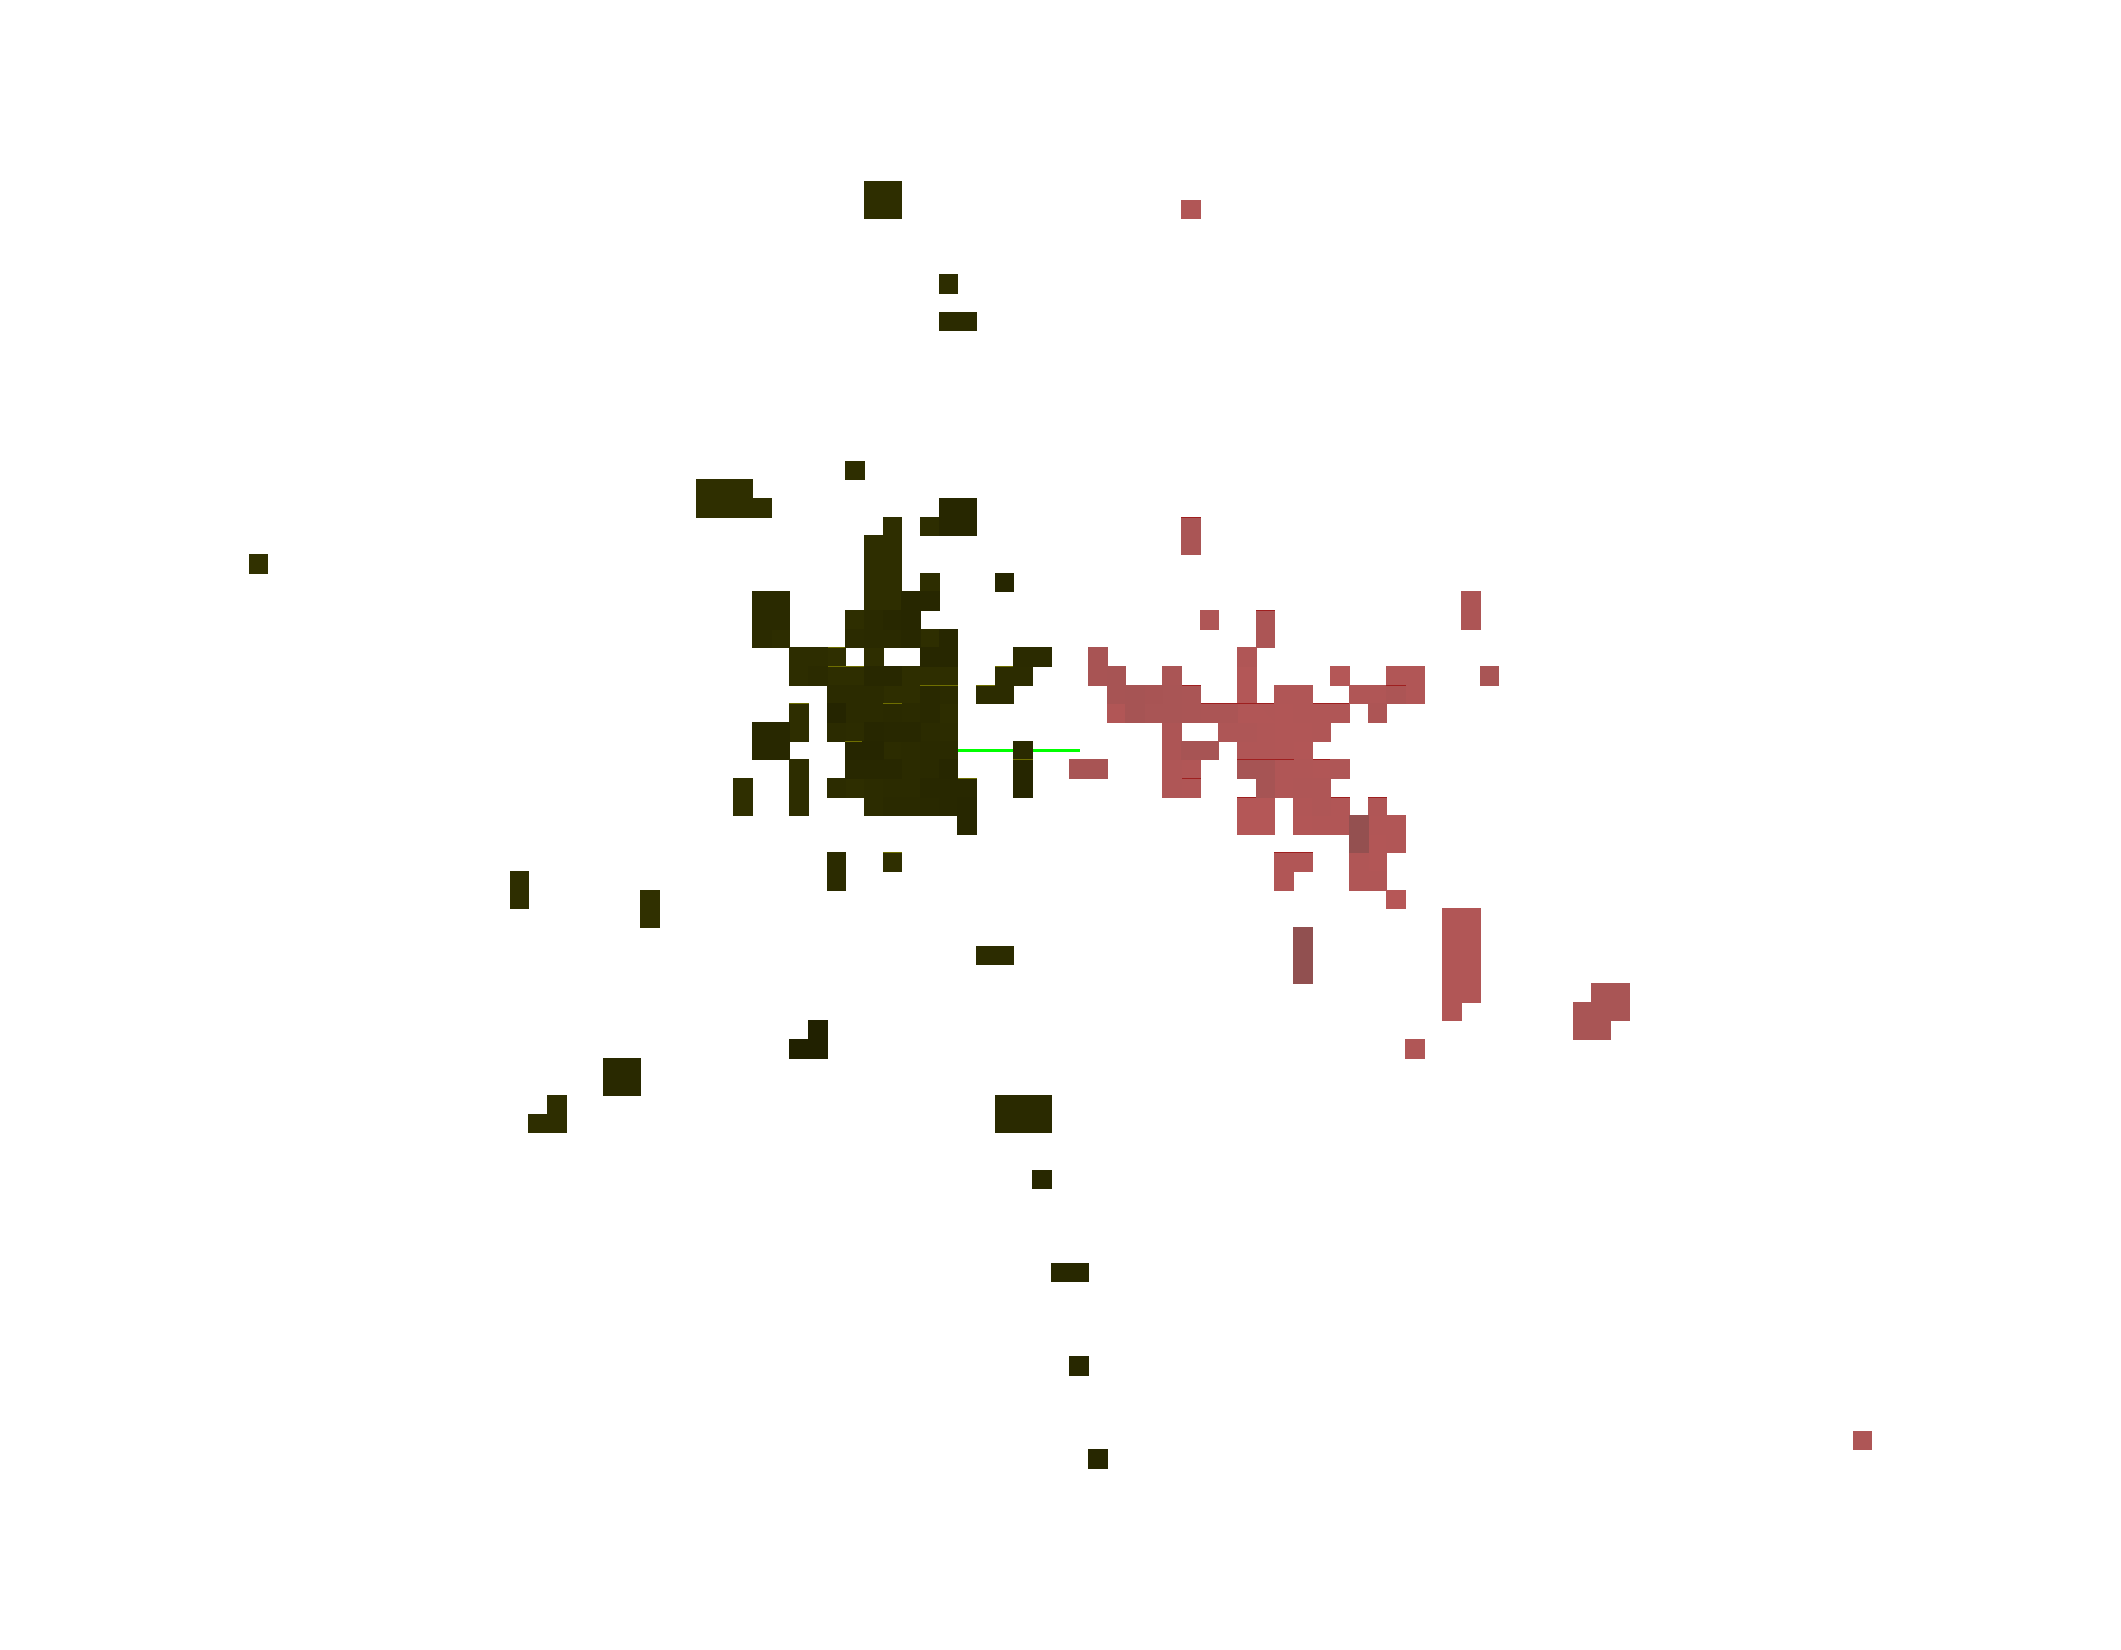
\includegraphics[width=0.32\linewidth]{ArborPFA_PandoraMonitoring_SDHCAL_Overlay_XY.pdf}
    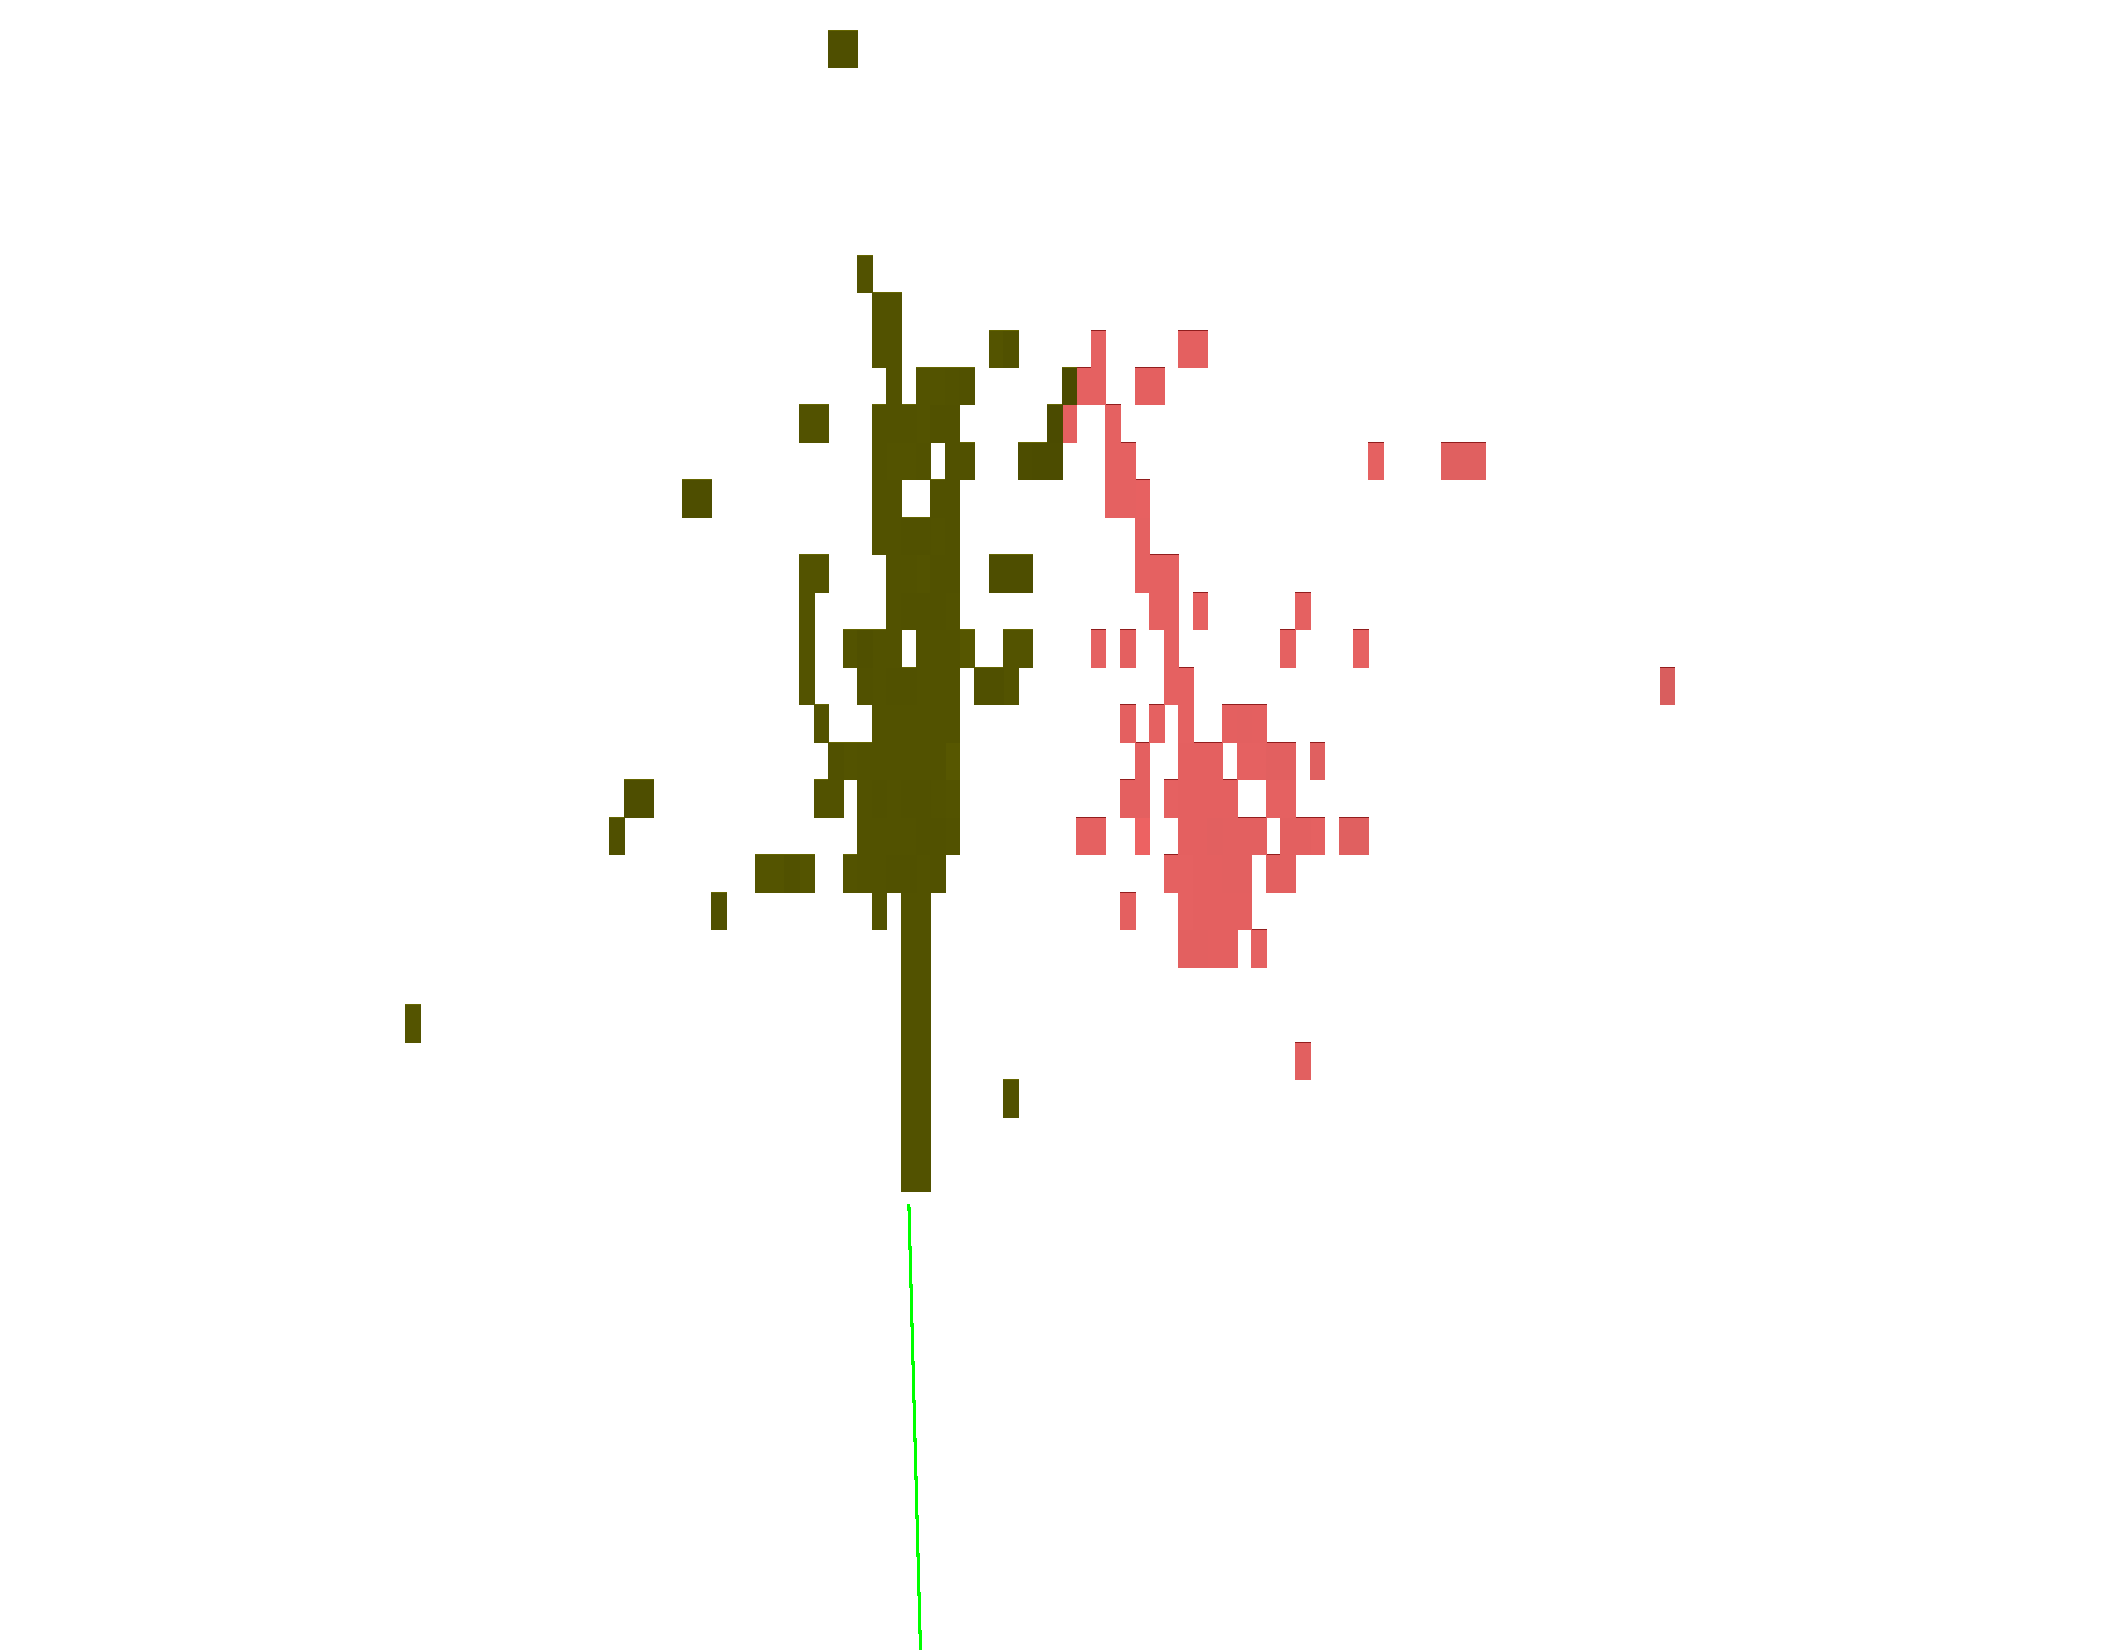
\includegraphics[width=0.32\linewidth]{ArborPFA_PandoraMonitoring_SDHCAL_Overlay_XZ.pdf}
    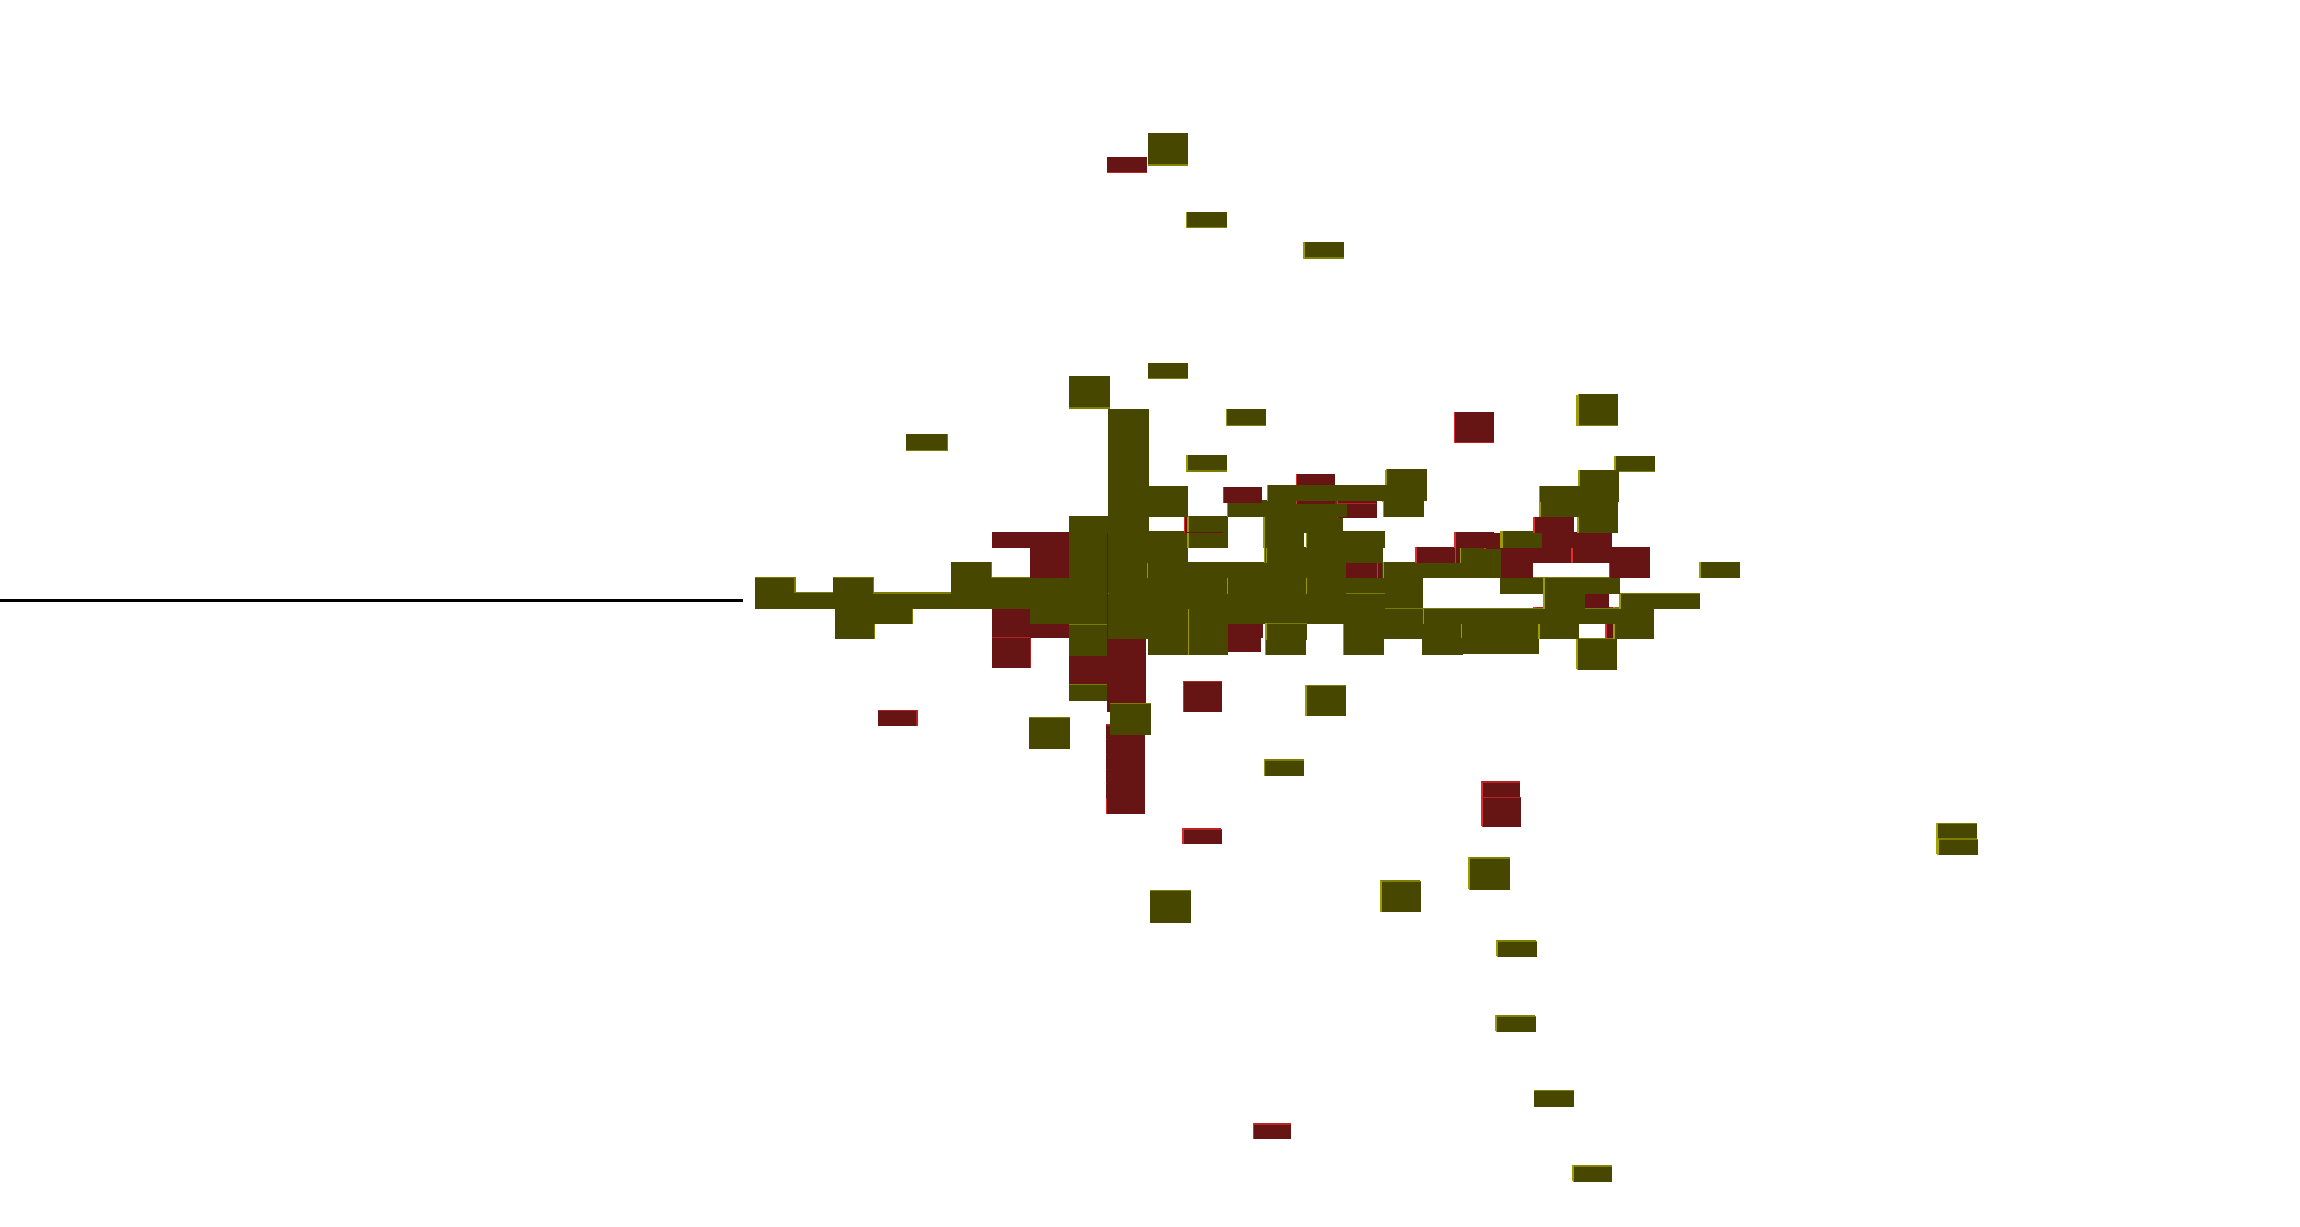
\includegraphics[width=0.32\linewidth]{ArborPFA_PandoraMonitoring_SDHCAL_Overlay_YZ.pdf}
  \end{center}
  \caption{\label{OVERLAY_EVENT_DISPLAY} Display of a 10 GeV fake neutral hadron overlaid with a 30 GeV charged hadron separated by 20 cm in three different views (XoY on left, XoZ in center and YoZ on right). Colours correspond to the reconstructed PFOs after running the ArborPFA program. The black straight line is the fake track generated in front of the calorimeter.}
\end{figure}

\subsection{Overlaid particles analysis}

\begin{figure}[!h]
  \begin{center}
    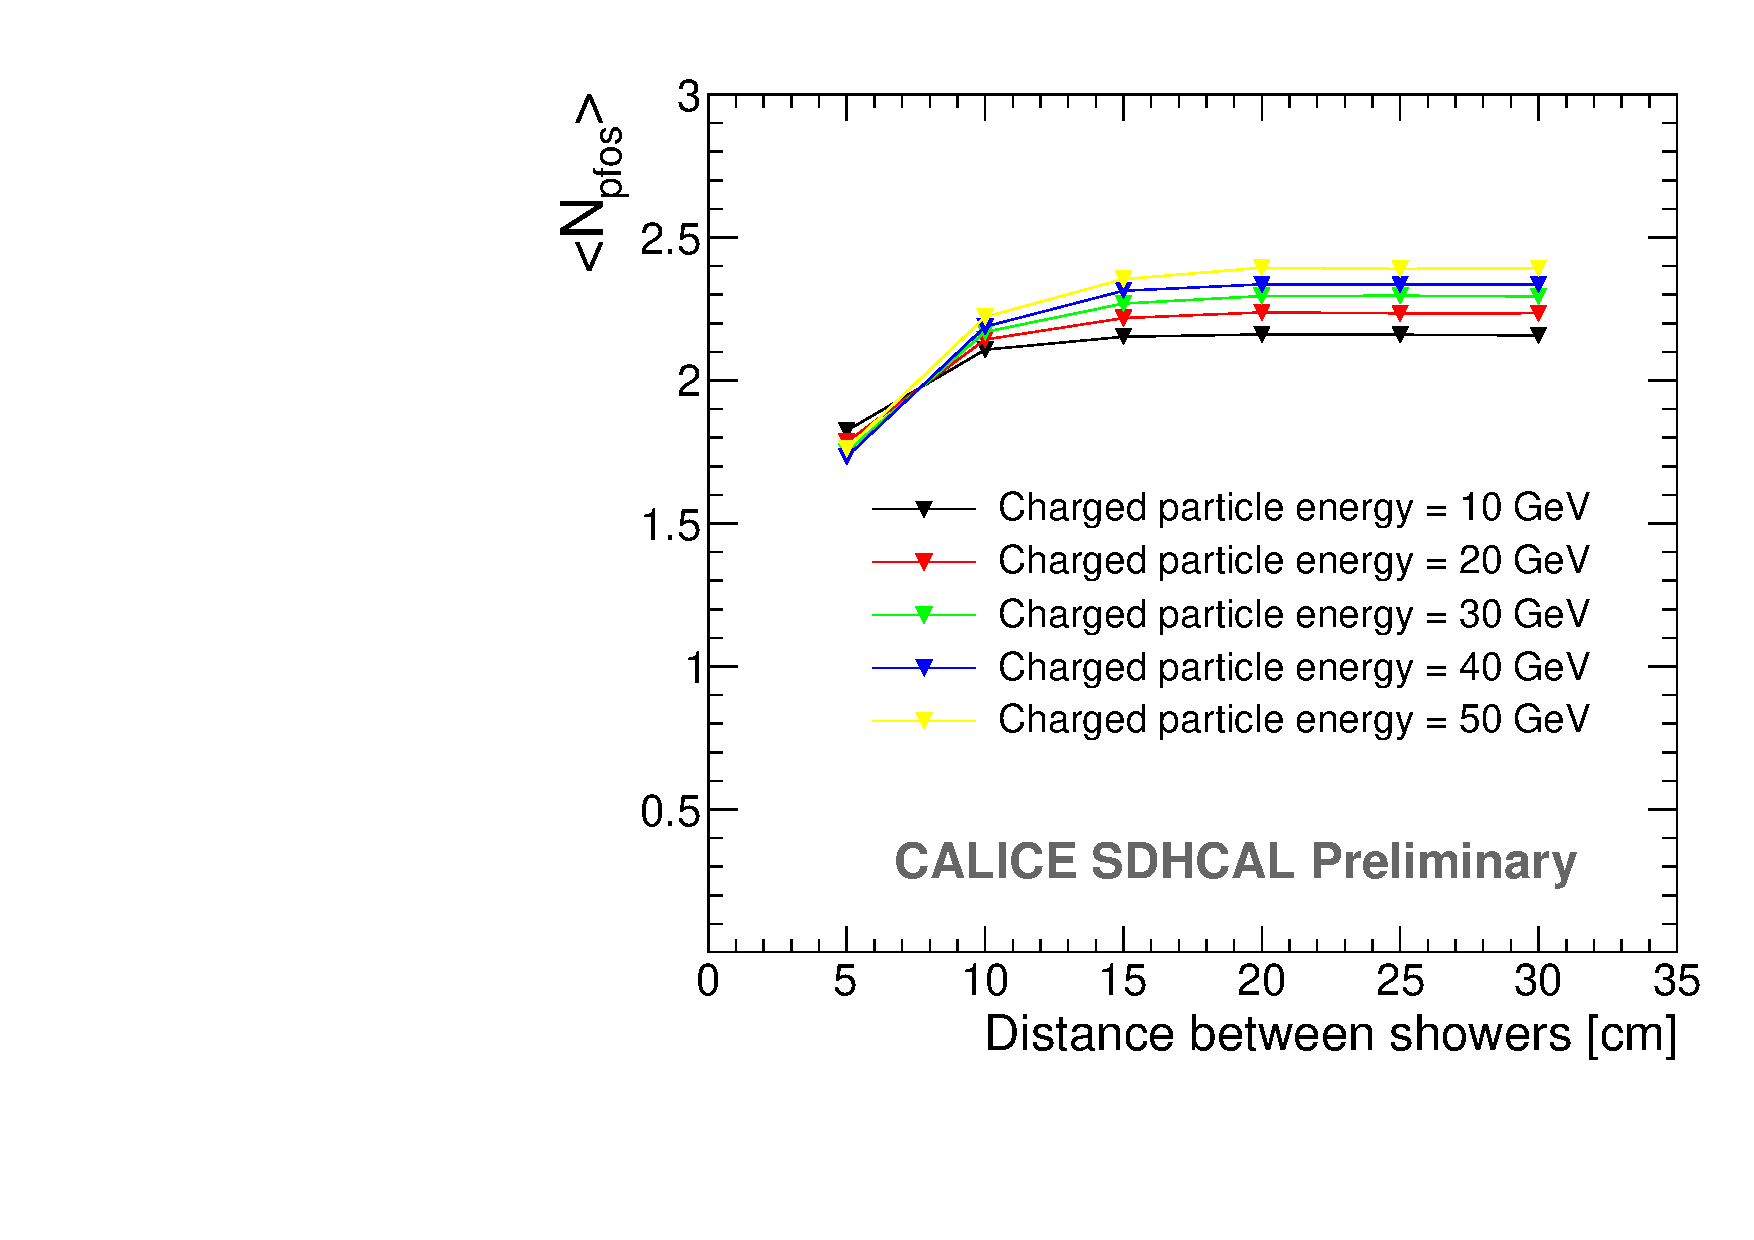
\includegraphics[width=0.6\linewidth]{plots/OverlayEvent_NPfos.pdf}
  \end{center}
  \caption{\label{OVERLAY_EVENT_NPFOS} The mean number of PFOs after running the ArborPFA program on overlaid particles.}
\end{figure}


Figure \ref{OVERLAY_EVENT_NPFOS} shows the mean number of PFOs after running the ArborPFA program on a 10 GeV fake neutral hadron overlaid with a charged hadron at different energies and different separation distances. The behaviour at a large separation distances where the number of PFOs increases with the charged particle energy matches the behaviour of the number of PFOs in the single particle study. We can also see that the sum of the number of PFOs for the single particle is compatible with the number of PFOs for the overlay. The mean number of PFOs is stable at large separation distances but slightly decreases at 5 cm from about 2.1 PFOs down to about 1.8 PFOs due to the showers overlaps and resulting confusions.

\begin{figure}[!h]
  \begin{center}
    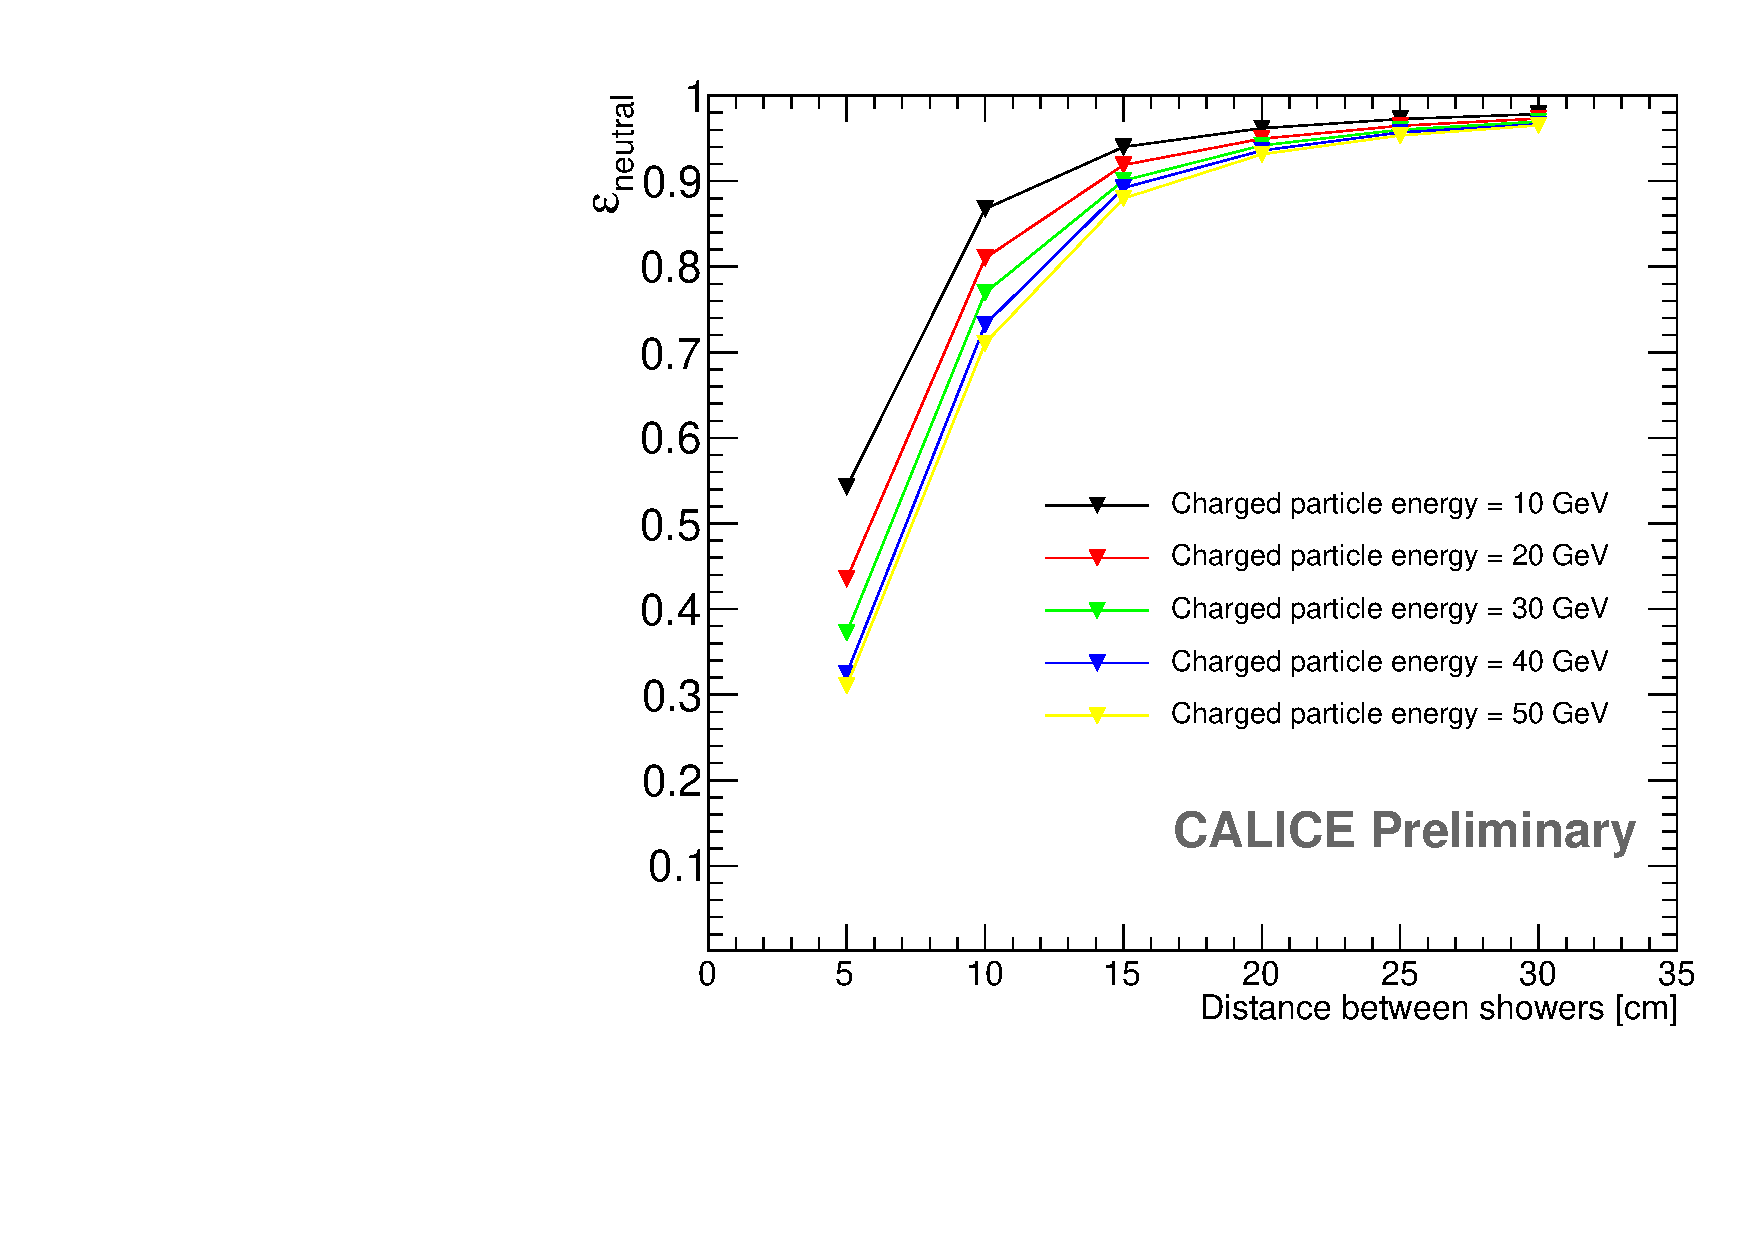
\includegraphics[width=0.47\linewidth]{plots/OverlayEvent_NeutralEfficiency.pdf}
    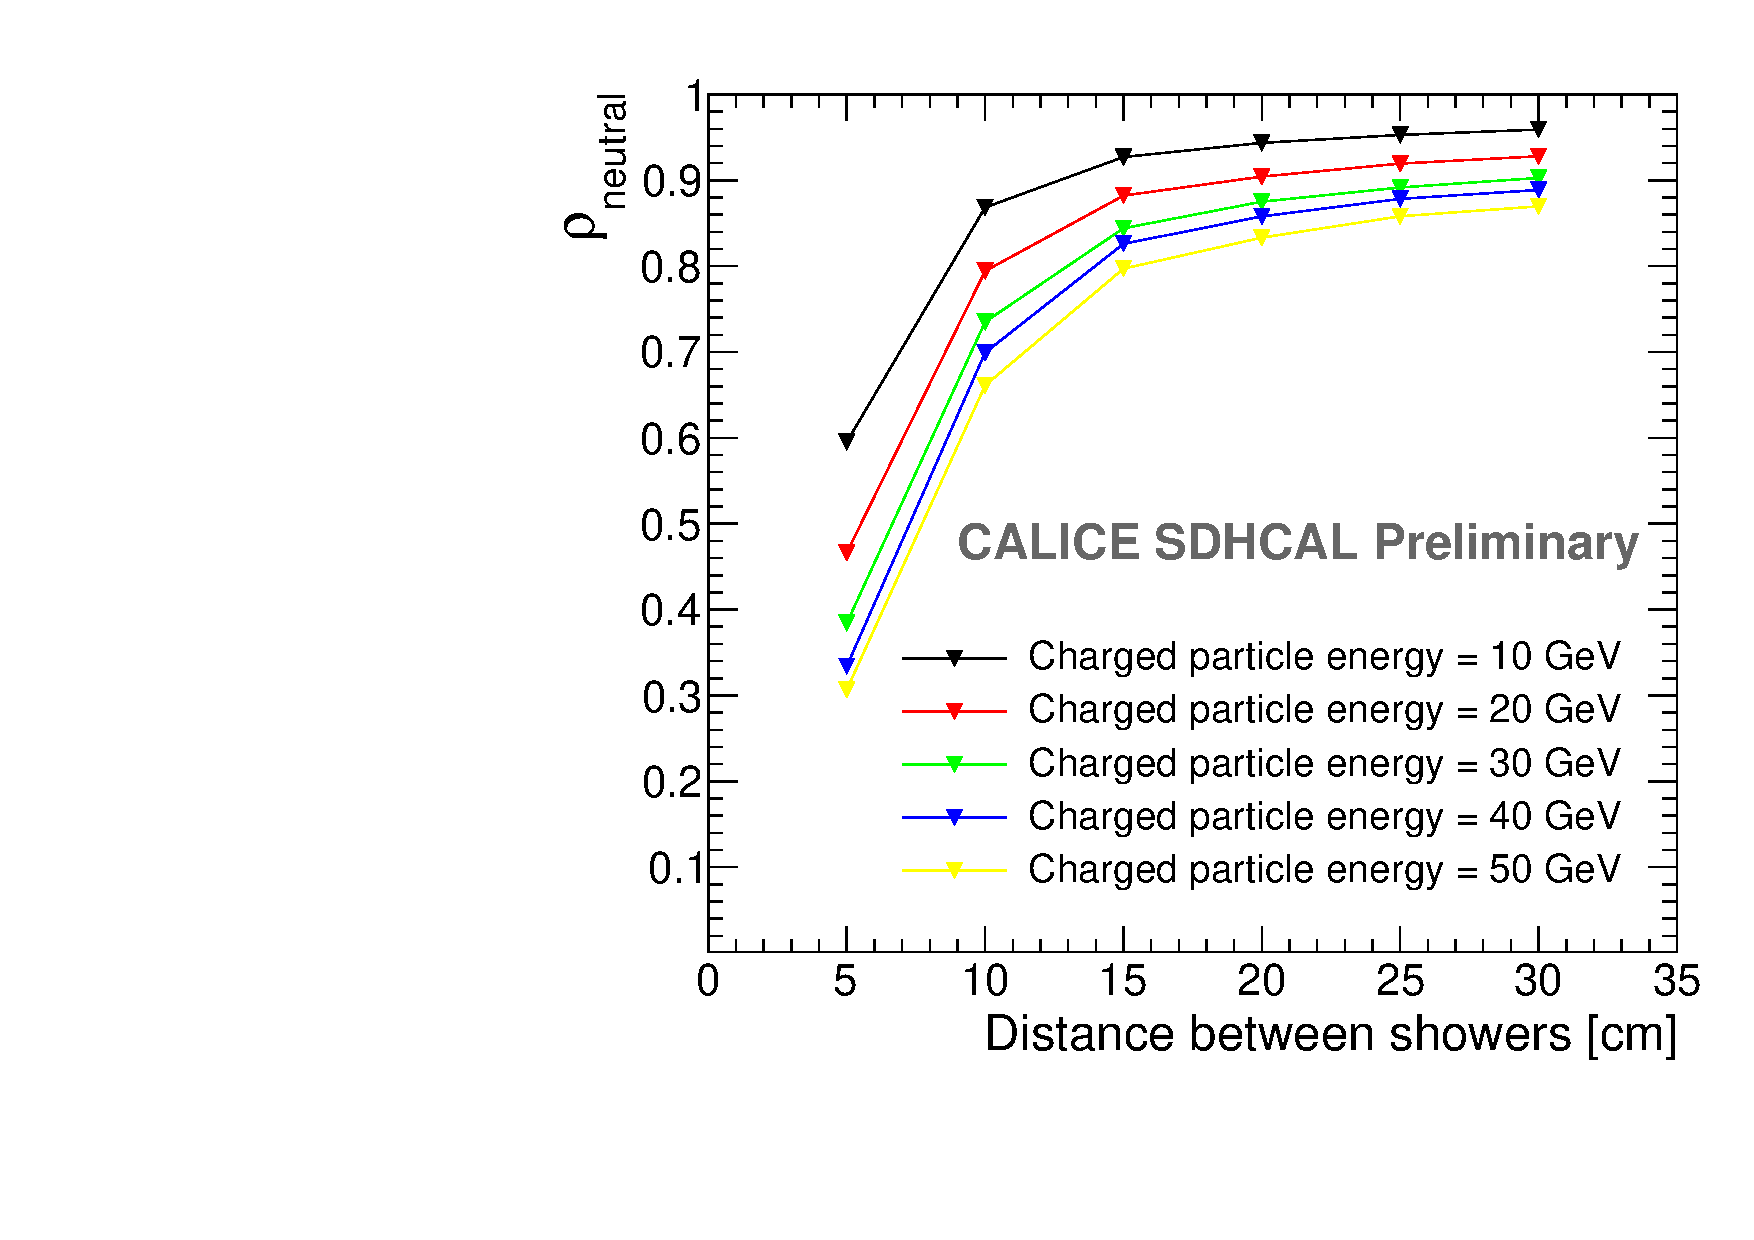
\includegraphics[width=0.47\linewidth]{plots/OverlayEvent_NeutralPurity.pdf}
  \end{center}
  \caption{\label{OVERLAY_EVENT_PURITY_EFFICIENCY} The efficiency (left) and purity (right) of the 10 GeV neutral hadron after reconstruction}
\end{figure}


To quantify the separation, we define the efficiency and the purity related to the reconstruction of one of the two related showers as :

\begin{equation}
  \epsilon = \frac{Nhit_{good}}{Nhit_{ini,tot}}
\end{equation}
\begin{equation}
  \rho = \frac{Nhit_{good}}{Nhit_{rec,tot}}
\end{equation}

with Nhit$_{good}$ the number of hits that initially belong to the particle and correctly assigned after reconstruction, Nhit$_{rec,tot}$ the total number of hits of the reconstructed shower and Nhit$_{ini,tot}$ the total number of hits of the particle before reconstruction. 

Figure \ref{OVERLAY_EVENT_PURITY_EFFICIENCY} shows the efficiency (left) and the purity (right) of the neutral hadron for different charged particle energies and different separation distances. In the same way as for the mean number of PFOs, at small distances the two showers start to overlap and confusions appear in the reconstruction. Thus, some hits of the neutral hadron are assigned to the charged one (and vice versa) and the efficiency and purity decrease. At large separation distances, the purity does not tend to 100\%. This is due to the last performed algorithm (small neutral fragment algorithm) which merges small neutral cluster fragments to their closest parent cluster, without considering the parent cluster size or energy. Since the number of neutral fragments for a single hadron particle increases with the energy, a non-negligible part of the charged hits is assigned to the neutral hadron, leading to a decrease of its purity.

Figure \ref{OVERLAY_EVENT_NEUTRAL_PERCENTAGE} (left) shows the fraction of events in which at least one neutral hadron has been reconstructed. As expected, the number of reconstructed neutral particles decreases with the separation distance. From 30 cm down to 15 cm, this fraction is stable and greater than 97\%. At 10 cm, confusions becomes significant and the neutral hadron is sometimes merged with the charged one, leading to a small decrease of this fraction. At 5 cm, we can see that the fraction strongly depends on the charged particle energy and goes from 73\% of reconstructed events for the 10 GeV charged particle case down to 60\% at 50 GeV.

\begin{figure}[!h]
  \begin{center}
    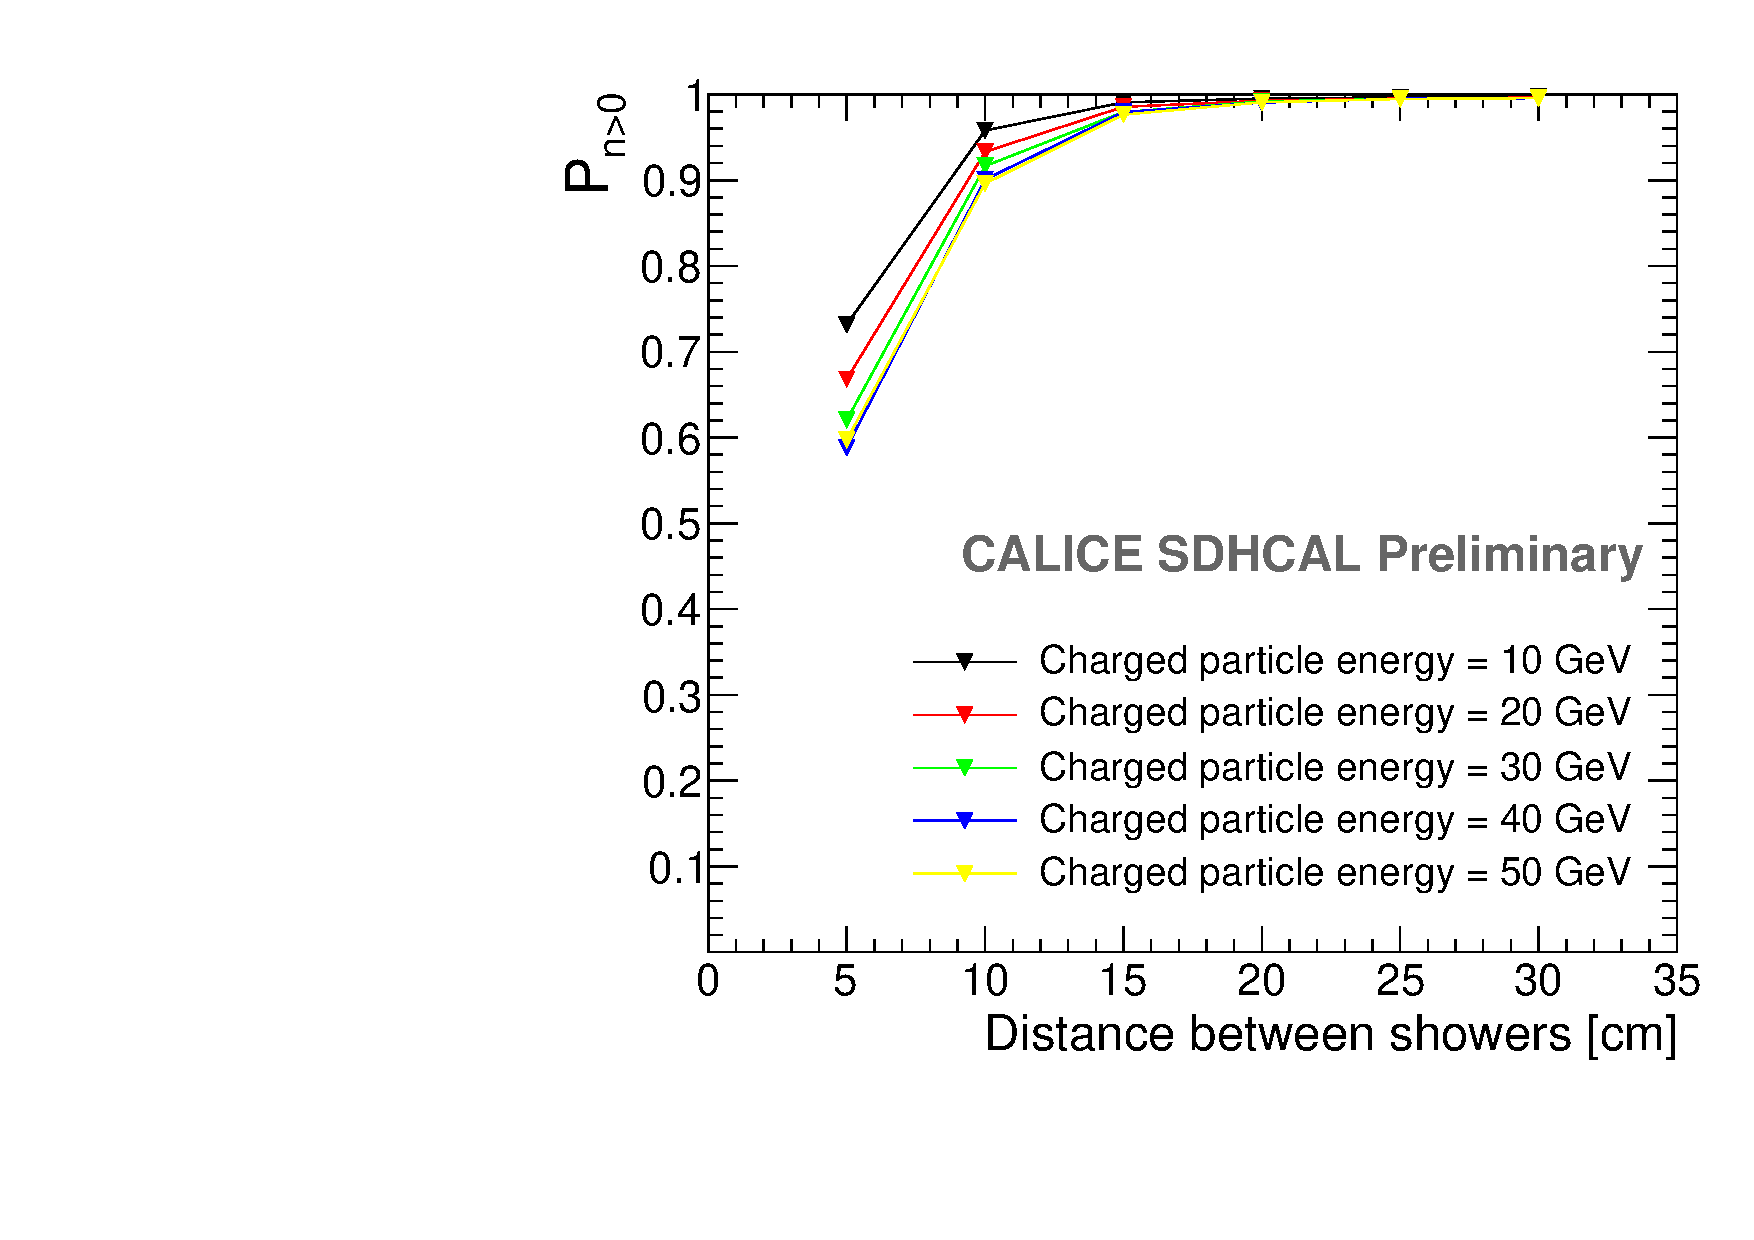
\includegraphics[width=0.47\linewidth]{plots/OverlayEvent_NeutralPercentage.pdf}
    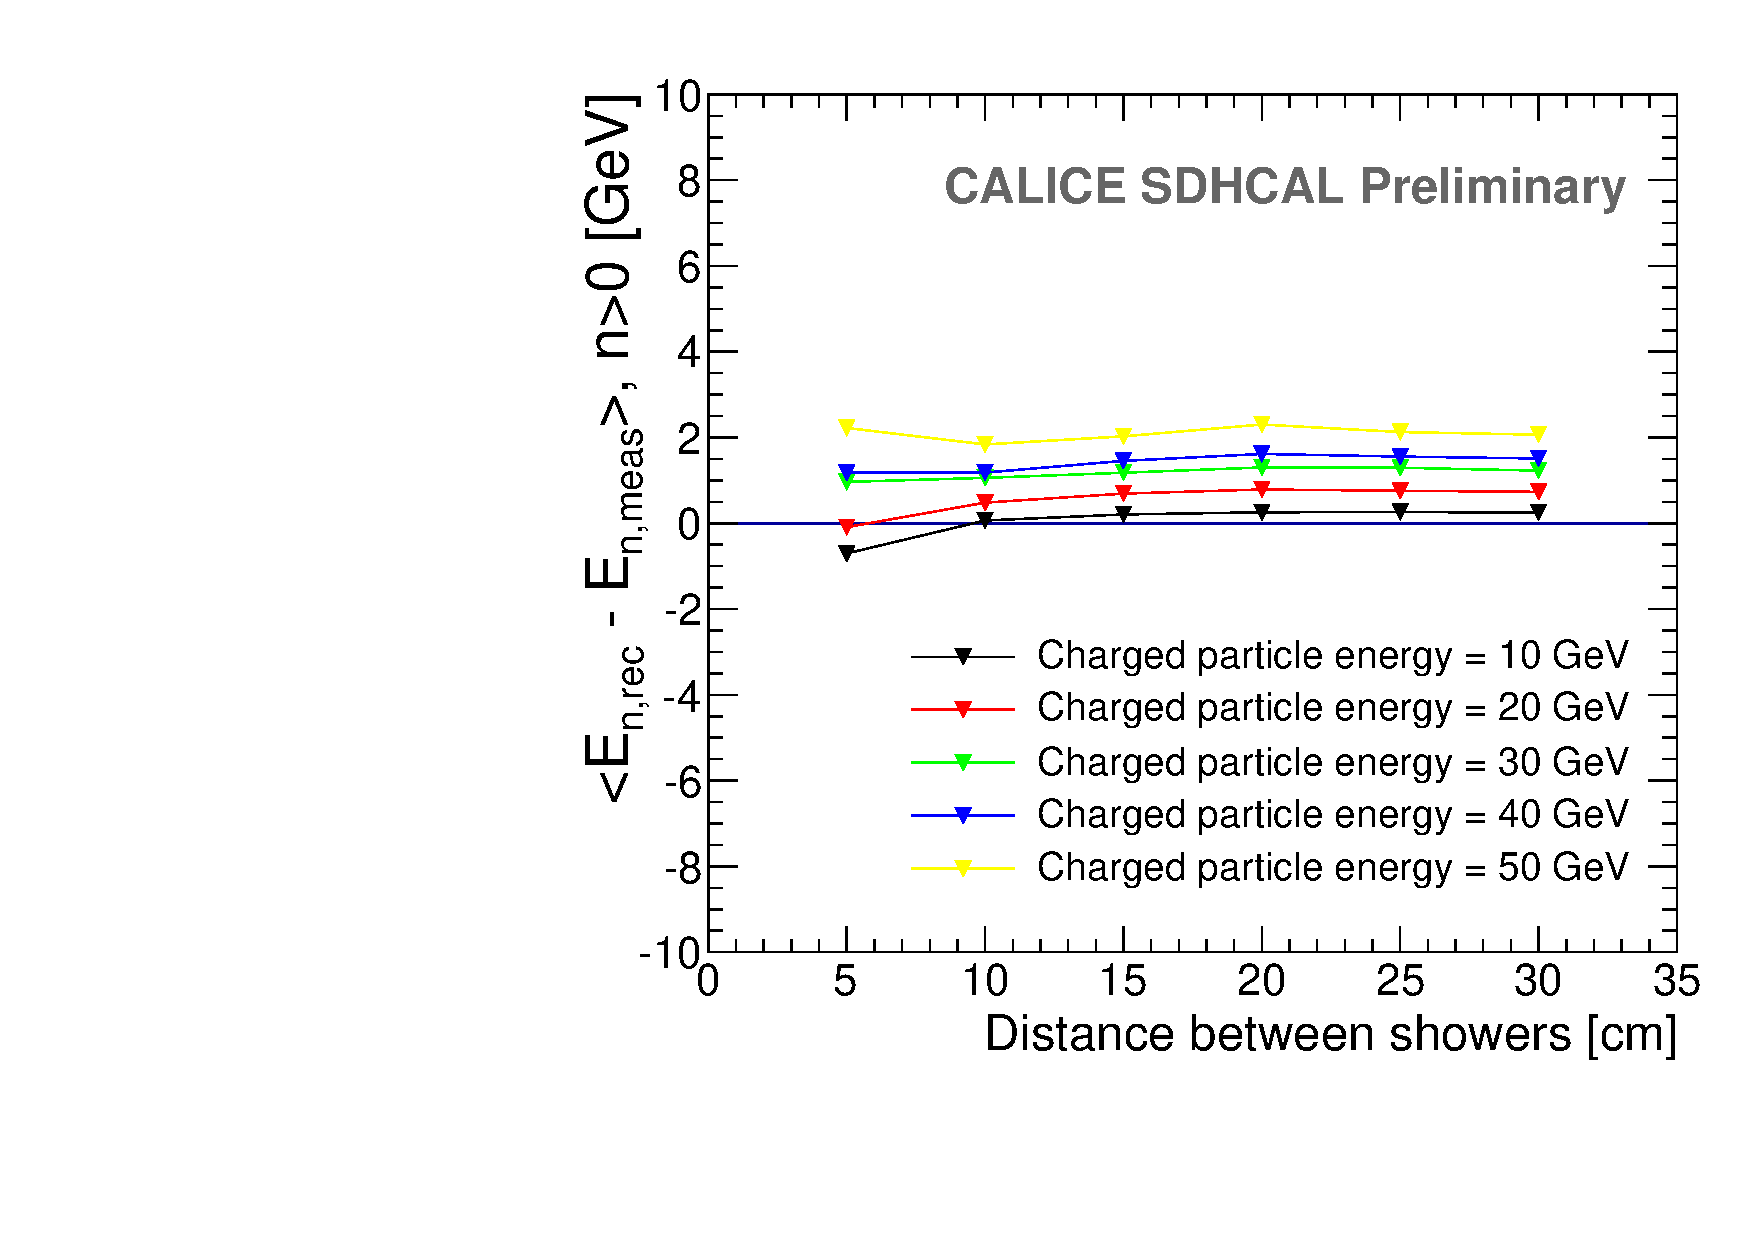
\includegraphics[width=0.47\linewidth]{plots/OverlayEvent_NeutralEnergyDifferenceMeanNeutralEfficient.pdf}
  \end{center}
  \caption{\label{OVERLAY_EVENT_EREC} \label{OVERLAY_EVENT_NEUTRAL_PERCENTAGE} Left : The fraction of events where at least one neutral hadron has been reconstructed. Right : The mean difference between the reconstructed energy and the measured energy before reconstruction for which at least one neutral hadron has been reconstructed.}
\end{figure}

We define the reconstructed neutral energy as the sum of the neutral particle energies and the measured neutral energy as the estimated energy before reconstruction. Figure \ref{OVERLAY_EVENT_EREC} (on the right) shows the mean difference between the reconstructed neutral energy and the measured neutral energy when at least one neutral hadron has been reconstructed. In the same way as for the purity, the mean reconstructed neutral energy increases with the charged particle energy. This plot also shows a flat behavior of the reconstructed neutral energy with the separation distance. This means that the reconstruction of the neutral hadron at very small distance (5 cm) has a \textit{binary-like} behaviour, either well reconstructed or completely merged with the charged hadron.

%%%%%%%%%%%%%%%%%%%%%
%%%%%% Summary %%%%%%
%%%%%%%%%%%%%%%%%%%%%
\newpage
\section{Summary}

The ArborPFA, based on the tree-like structure of hadronic showers has been described in details. 

A single particle study has been performed on SDHCAL test beam data taken at SPS at CERN during August and September 2012 \cite{sdhcal-paper}. Single pion showers have been selected and a track in front of the calorimeter has been created in order to emulate a track from a tracking detector.

The results show a good efficiency with more than 95\% of hits assigned to the reconstructed charged particle over the energy range of 10 to 80 GeV. The mean number of PFOs shows a linear increase with the energy from 1.1 PFOs at 10 GeV to 1.4 PFOs at 80 GeV. Around 4\% of hits are not clustered by the algorithm, leading to a small decrease in the clustered energy response and a small degradation of the energy resolution with respect to the case in which all hits are considered.

The ability of the algorithm to separate nearby hadronic showers was also investigated. Two different charged hadron showers with different energies from the same test beam data set have been overlaid in the same event with different separation distances. For the 10 GeV pion shower, the track segment inside the calorimeter has been identified and removed from the event in order to emulate a neutral hadron particle. For the other particle, a track has been generated in front of the calorimeter and pointing on the particle entry point, as for the single particle case. 

The results showed a neutral hadron recovery higher than 90\% until 10 cm separation distance where a non negligible confusion starts to appear. 

The difference between the reconstructed energy and the measured energy of the neutral hadron in the case where at least one neutral hadron has been reconstructed showed an increase with the charged hadron energy for all the separation distances due to the small neutral fragment merging algorithm. At small separation distance (5cm), the difference stays constant and shows that the neutral hadron reconstruction has a \textit{binary-like} behaviour, either a very good reconstruction or merged in the charged hadron.

This work will be extended shortly to include the electromagnetic calorimeter as well as the other sub-detectors in the framework of the ILD detector with the aim to separate charged and neutral hadrons produced in jets to improve on the PFA performances.

\newpage
\begin{thebibliography}{6}
\renewcommand{\hepex}[1]{\href{http://www.arxiv.org/abs/#1}{\tt hep-ex/#1}}
\renewcommand{\physics}[1]{\href{http://www.arxiv.org/abs/#1}{\tt phys.int-det/#1}}
\newcommand\nim[4]{\href{http://dx.doi.org/10.1016/#4}
  {\emph{Nucl.\ Instrum.\ Meth.} {\bf #1} (#2) #3}}
\newcommand\can[1]{\href{https://twiki.cern.ch/twiki/pub/CALICE/CaliceAnalysisNotes/CAN-#1.pdf}{\tt CAN-#1}}


\bibitem{sdhcal-paper} 
Calice Collaboration, \emph{First results of the CALICE SDHCAL technological prototype}, \can{037}

\bibitem{ilc-tdr} 
J. Carwardine {\it et al.},  \emph{International Linear Collider Technical Design Report}. 1) Executive Summary, 2) Physics, 3) Accelerator, 4) Detectors. 12 June 2013

\bibitem{hadron-jets} 
O. Lobban, A. Sriharan, R. Wigmans,  \emph{On the energy measurement of hadron jets}, \nim{A495}{2002}{107-120}

\bibitem{marlin-lccd}
F. Gaede, Marlin and LCCD: Software tools for the ILC, \nim{A559}{2006}{177-180}

\bibitem{pandora-pfa}
M. A. Thomson, \emph{Particle Flow Calorimetry and the PandoraPFA Algorithm}, \physics{0907.3577}

\bibitem{pandora-sdk}
J. S. Marshall, M. A. Thomson, \emph{The Pandora Software Development Kit for Pattern Recognition}, \physics{1506.05348}

\bibitem{arbor-manqi}
M. Ruan, \emph{Arbor, a new approach of the Particle Flow Algorithm}, Proceeding of CHEF 2013. \hepex{1403.4784}

\bibitem{ilcsoft}
ILCsoft, 2012. \href{http://ilcsoft.desy.de/portal}{\tt http://ilcsoft.desy.de/portal}

\bibitem{root}
ROOT, 1995-2015, \href{https://root.cern.ch/drupal}{\tt https://root.cern.ch/drupal}

\newpage

\end{thebibliography}


\clearpage
\appendix

\section{ArborPFA algorithm}
\label{ARBOR_ALGO_DESCRIPTION}

Before describing the algorithm in detail, a few definitions specific to ArborPFA need to be introduced :

\paragraph*{Object} An \textit{object} is a calorimeter hit or a group of contiguous calorimeter hits within a layer that serves as a vertex for the ArborPFA algorithm. This was introduced for two reasons i) to provide a generalization of connections between \textit{objects} without making any assumptions of what is contained in an \textit{object}, ii) to overcome the pad multiplicity\footnote{More than one pad could be fired when a particle crosses the gas gap.} inherent in the SDHCAL \cite{sdhcal-paper} and similar detectors.

\paragraph*{Flow direction} The flow direction is of two kinds : forward direction which is from upstream to downstream of the beam direction and backward direction for the opposite.

\paragraph*{Connector} A connector is a link between two \textit{objects}. It has a weight and a direction.

\paragraph*{Connector depth} The connector depth is defined as the number of intermediary connectors linking two different objects.

\paragraph*{Tree} A tree is a set of \textit{objects} connected in a tree topology, which means that for each object there is only one backward connector. An \textit{object} without a backward connector is called a seed and an \textit{object} without a forward connector is called a leaf.

\paragraph*{Cluster} A cluster is a set of trees.

\paragraph*{Particle flow object (PFO)} A particle flow object is a set of clusters and tracks \footnote{By \textit{track} we mean one reconstructed by a tracking detector such as a TPC}, which corresponds to a reconstructed particle.

~\newline 
Note that in the following algorithm descriptions, some parameters are labelled by a name or symbol, whose values are given in a separate Appendix \ref{ARBOR_ALGORITHM_PARAMETERS}.

\subsection*{Pre-clustering phase} 
%%%%%%%%%%%%%%%%%%%%%%%%%%%%%%%%%%%%%%%%%%%

%%% OBJECT CREATION %%%
\begin{wrapfigure}{r}{0.4\textwidth}
  \vspace{-20pt}
  \begin{center}
    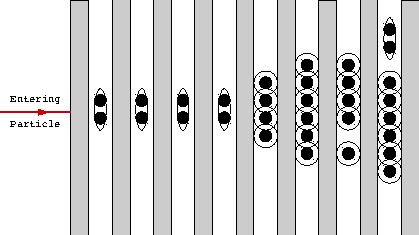
\includegraphics[width=\linewidth]{ObjectCreationAfter.pdf}
  \end{center}
  \vspace{-10pt}
  \caption{\label{ARBOR_OBJECT_CREATION} Schematic view of the object creation output. Small groups of contiguous calorimeter hits are grouped together (encircled).}
  \vspace{-20pt}
\end{wrapfigure}

~~~~~~~Before building trees, we need to create objects to connect with each other.

\paragraph*{Object creation} When a particle goes through the detector, several pads can be fired in a single layer, leading to a multiplicity greater than 1. To overcome this problem, intra-layer groups of hits are assembled using the nearest neighbour clustering algorithm (corner neighbours not included). If a group contains more than 4 hits, it is split and each individual hit is considered as a separate object. This generally happens in the shower core. If a group contains 4 or less hits, it is used to define a single object. This is the case for a mip or more generally any isolated non-showering particle. Figure \ref{ARBOR_OBJECT_CREATION} shows the output of this algorithm with encircled hits forming objects.

%%% MIP TAGGING %%%
\paragraph*{Track segment\footnote{By \textit{track segment} we mean a track produced by a charged particle in the calorimeter such as Minimum Ionizing Particles (MIP)} candidate tagging}
In order to correctly reconstruct the primary track segment in the calorimeter, track segment candidate \textit{objects} are identified and tagged for future treatment. For each object, we count the number of objects in the same layer within a distance of $\Delta_{mip}$. If this number doesn't exceed N$_{obj,cut}$, the object is tagged as a track segment candidate object.

\subsection*{The main clustering phase - Connectors and trees}
%%%%%%%%%%%%%%%%%%%%%%%%%%%%%%%%%%%%%%%%%%%

~~~~~~~The main clustering algorithm consists of an iterative procedure using dedicated algorithms to create and remove connectors (connector loop). At the end of this step, all objects are arranged in a tree structure, which means that each object has at most one connector in the backward direction and 0 or more in the forward direction.

\begin{figure}[!h]
  \begin{minipage}{0.49\linewidth}
    \begin{center}
      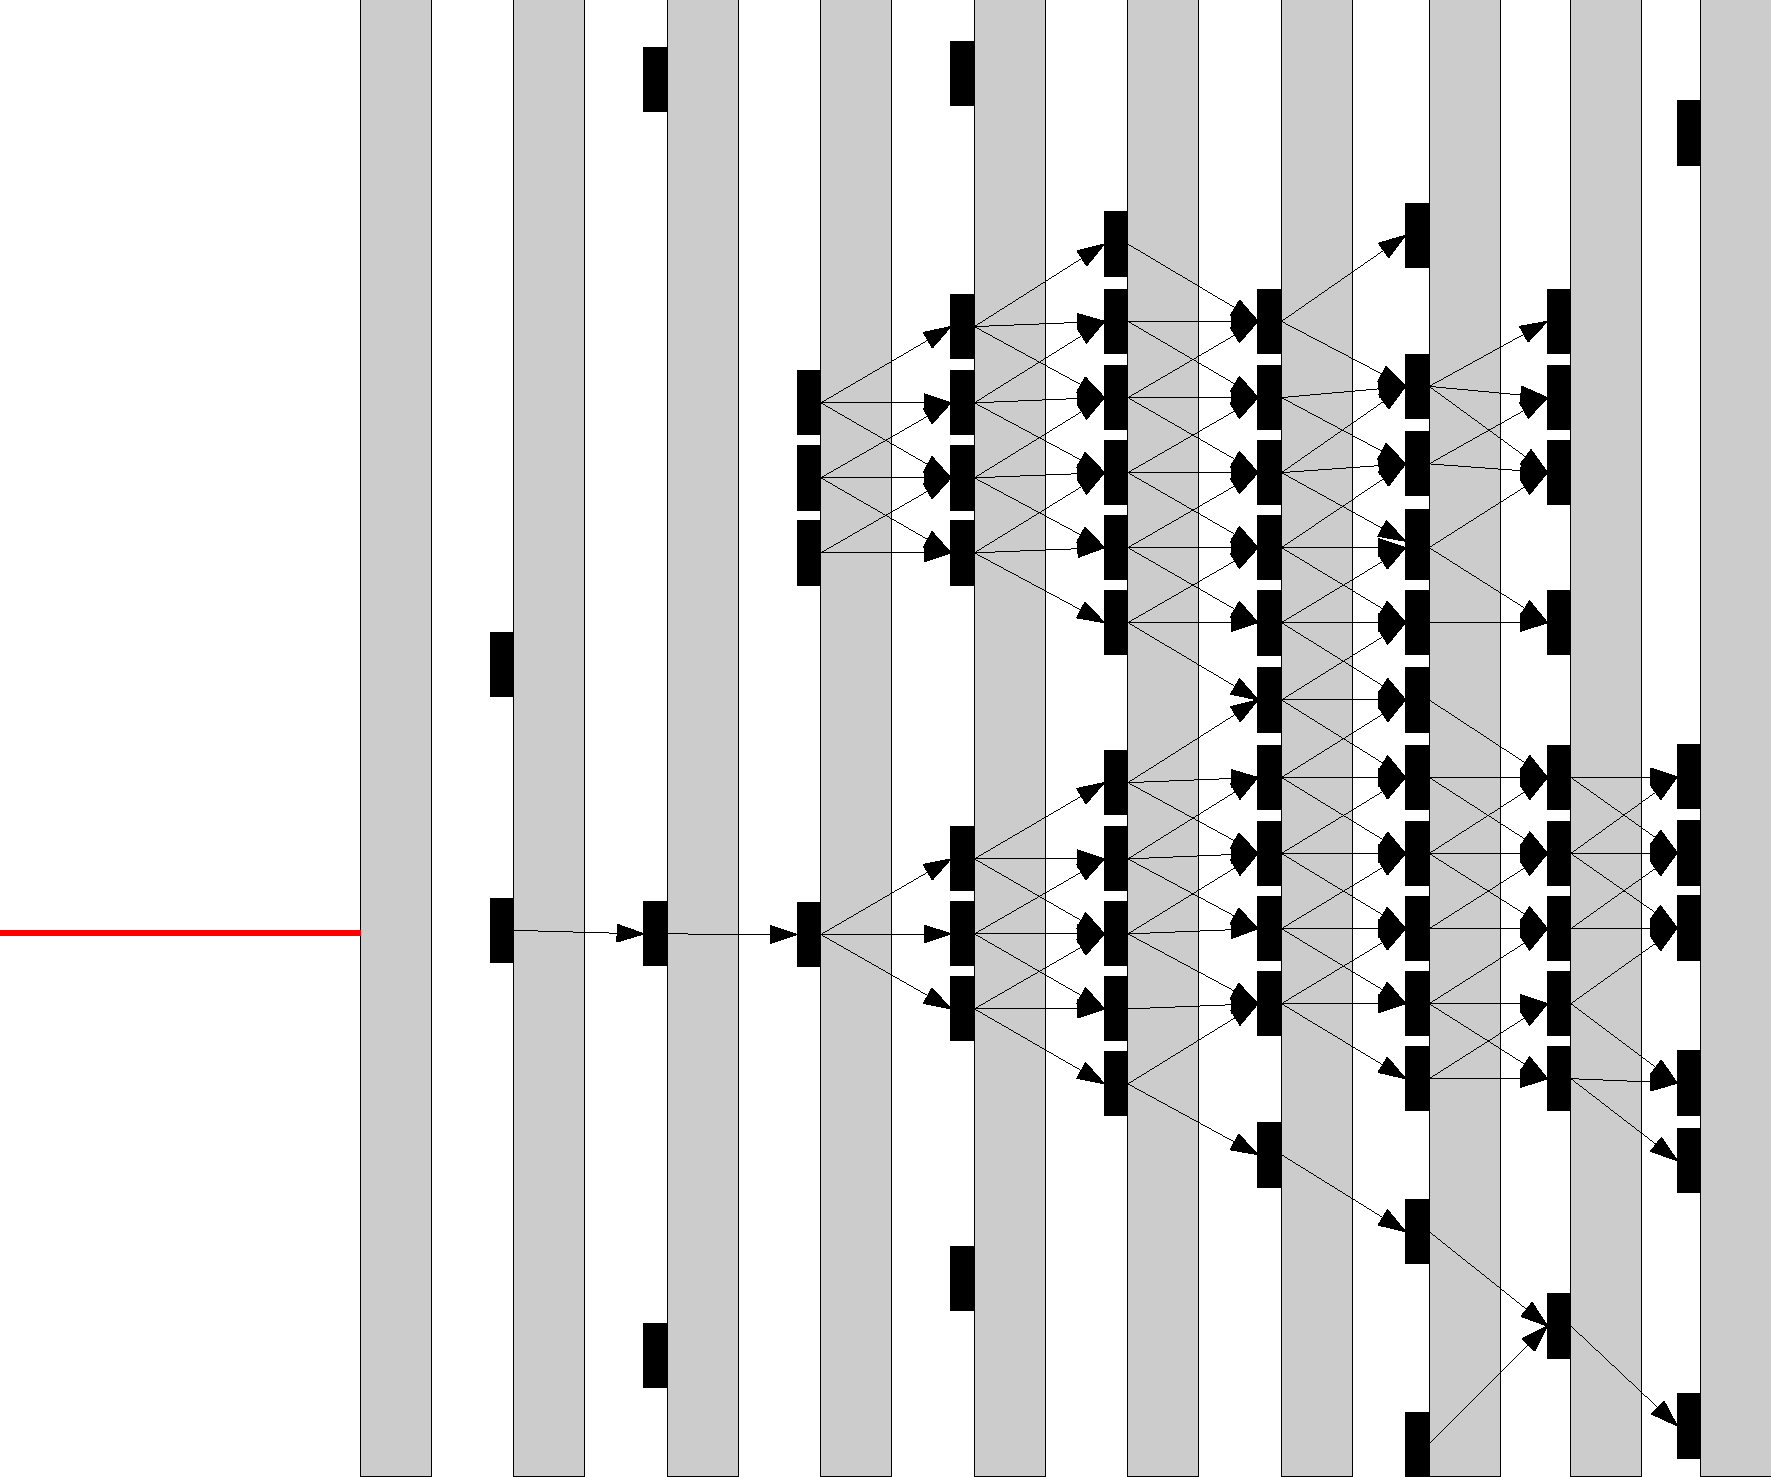
\includegraphics[width=0.9\linewidth]{ConnectorSeeding1.pdf}
    \end{center}
  \end{minipage}
  \begin{minipage}{0.49\linewidth}
    \begin{center}
      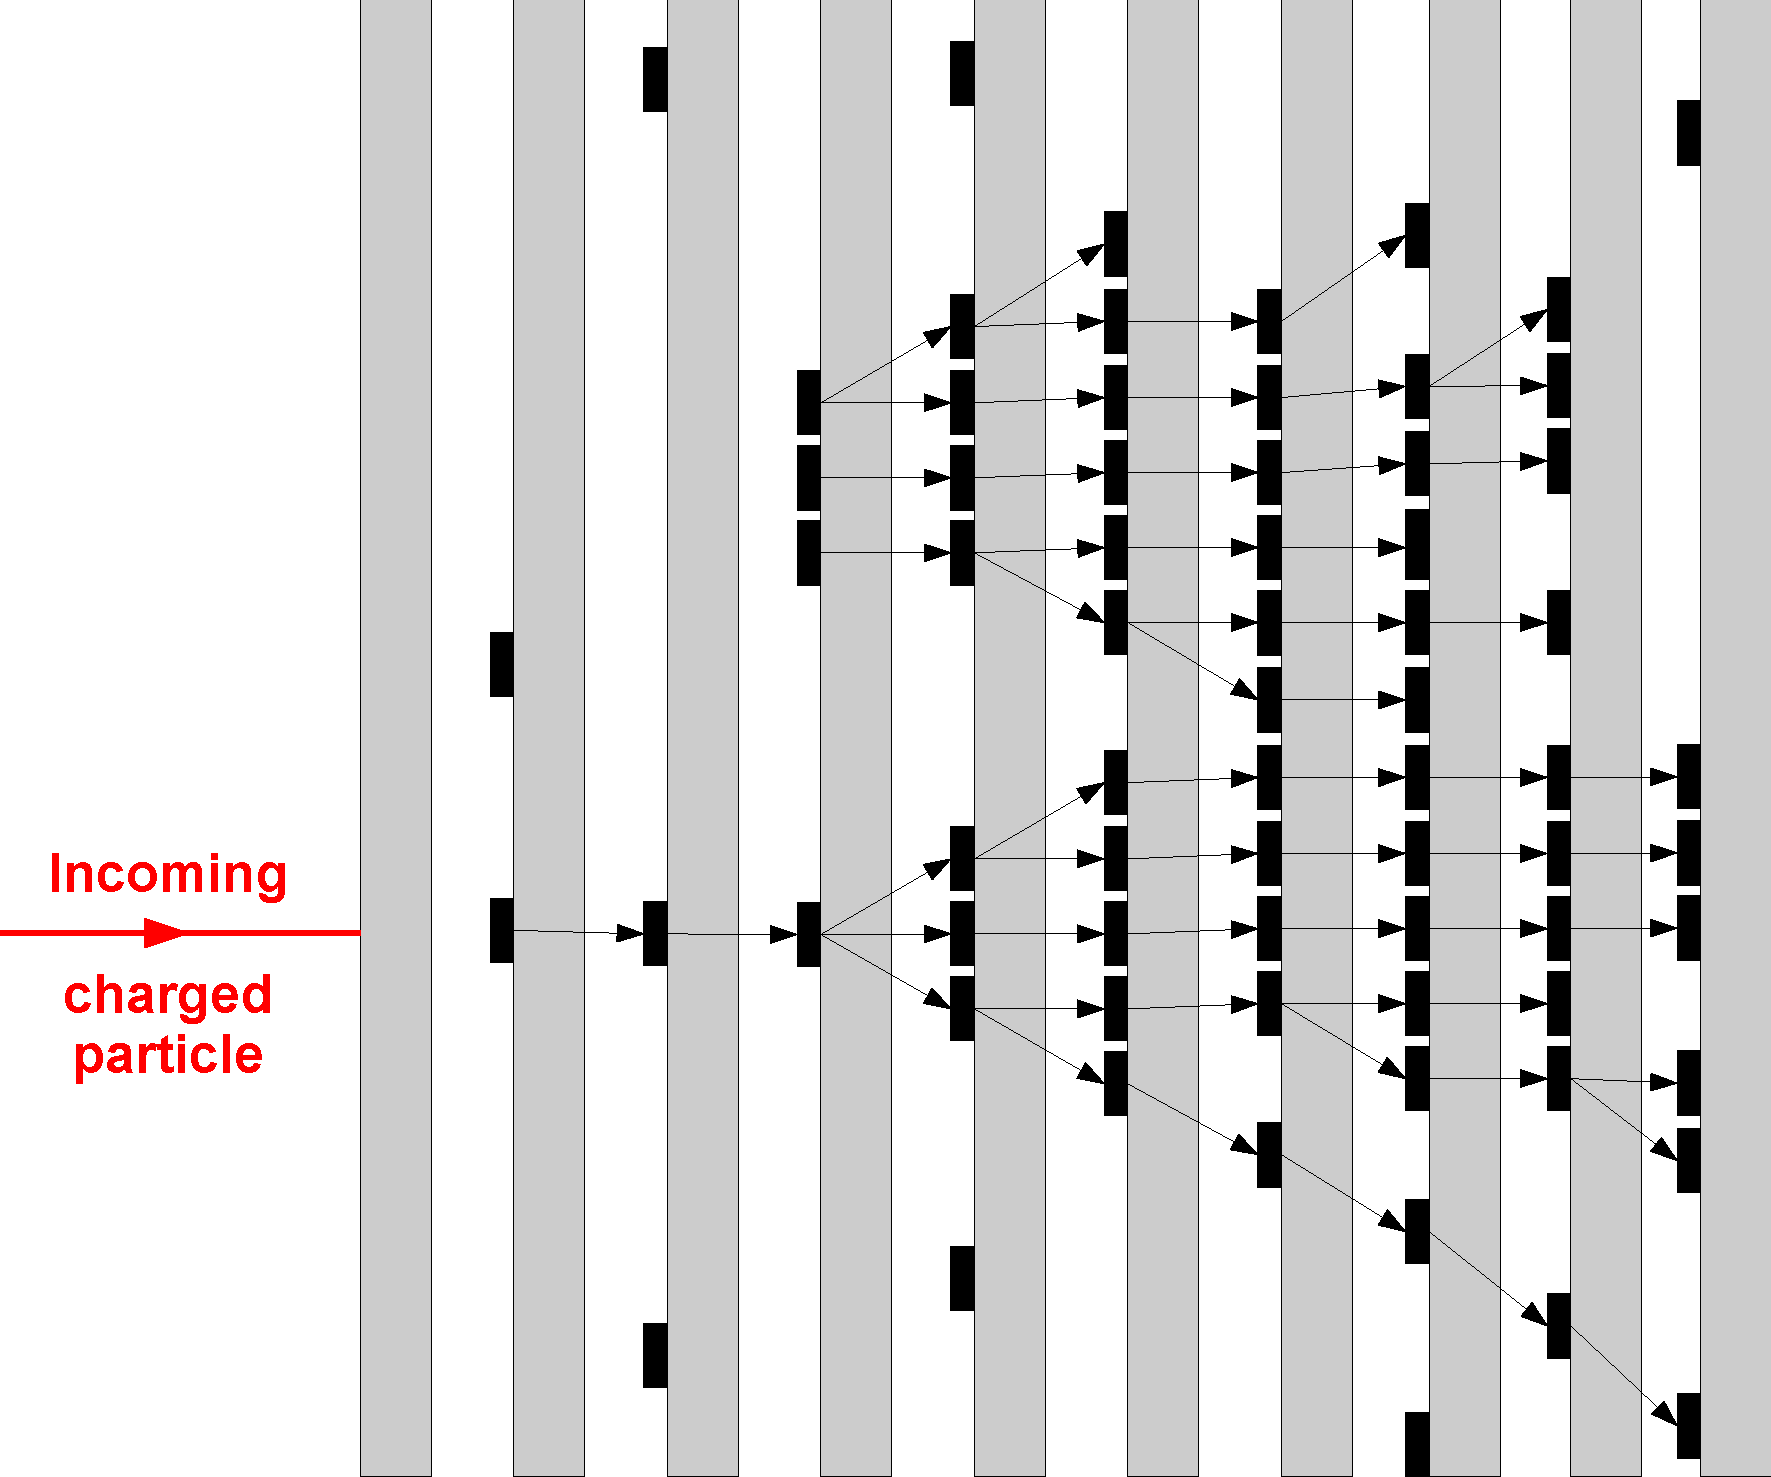
\includegraphics[width=0.9\linewidth]{ConnectorCleaning1.pdf}
    \end{center}
  \end{minipage}
  \caption{\label{ARBOR_CONNECTOR_SEEDING_1} \label{ARBOR_CONNECTOR_CLEANING_1} Schematic view of a neutral and a charged pion showers after the first connector seeding algorithm (left) and cleaning algorithm (right)}
\end{figure}

In the current implementation, the connector loop contains the following algorithms :

\paragraph*{Primary track connection} This algorithm aims to create connections between objects belonging to the primary track segment of charged particles in the calorimeter. It consists mainly in creating a sub-list of objects that are candidates for the primary track segments by using the objects tagged as track segment candidates and the track extrapolations on the front of the calorimeter. Once this list is built, the "\textit{connector seeding 1}" algorithm and the "\textit{connector cleaning 1}" algorithm are run on only the sub-list objects.

\paragraph*{Connector seeding 1} We start by creating connections in the neighbourhood of each object. For each object, we look for other objects in the N$_{layers}$ next layers within a maximum distance $\Delta_{max}$ and we create connections between them. As an example, Figure \ref{ARBOR_CONNECTOR_SEEDING_1} (left) illustrates the output of this algorithm.

\paragraph*{Connector cleaning 1} Once connectors are created, we need to build a tree structure by keeping only one connector in the backward direction for each object. We define the reference direction of an object as :

\begin{equation}
  \vec{C}_{ref} = w_{bck} . \sum_\sigma \sum_b \vec{c}_{b,\sigma} - w_{fwd} . \sum_\delta \sum_f \vec{c}_{f,\delta}
\end{equation}

where :

\begin{itemize}
  \item $w_{bck}$ ($w_{fwd}$) is a global positive weight assigned to backward (forward) connectors
  \item $\vec{c}_{b,\sigma}$ ($\vec{c}_{f,\delta}$) is the direction of a backward (forward) connector at the connector depth $\sigma$ ($\delta$) from the considered object
\end{itemize}

The depth parameter $\sigma$ has been fixed to 1 in all algorithms. The reference direction is a vector that goes in the backward direction and indicates the most probable direction for a unique backward connection. Then we need to assign which backward connector should be kept for the tree building. Thus, for each backward connector of an object, we define the $\kappa$ parameter as :

\begin{equation}
  \kappa~=~\Big(\frac{\theta}{\pi}\Big)^{p_{\theta}} . ~\Big(\frac{\Delta}{\Delta_{max}}\Big)^{p_{\Delta}} 
\end{equation}

where :

\begin{itemize}
  \item $\theta$ is the angle between a backward connector and the reference direction of the considered object,
  \item $\Delta$ is the distance between the connected objects,
  \item $p_{\theta}$ ($p_{\Delta}$) is a power parameter for the normalized angle (distance)
\end{itemize}

The $\kappa$ parameter quantifies the alignment with the reference direction within the range [0,1]. Smaller is this parameter, higher the alignment will be. The power parameters $p_{\theta}$ and $p_{\Delta}$ are to be tuned depending on which variable we want to emphasize.

The chosen backward connector for the tree building is the one with the smallest $\kappa$ parameter; all others are removed from the list. The removal of connectors is done at the end of the algorithm so that all connectors contribute to the evaluation of the reference direction.

\begin{figure}[!h]
  \begin{minipage}{0.4\linewidth}
    \begin{center}
      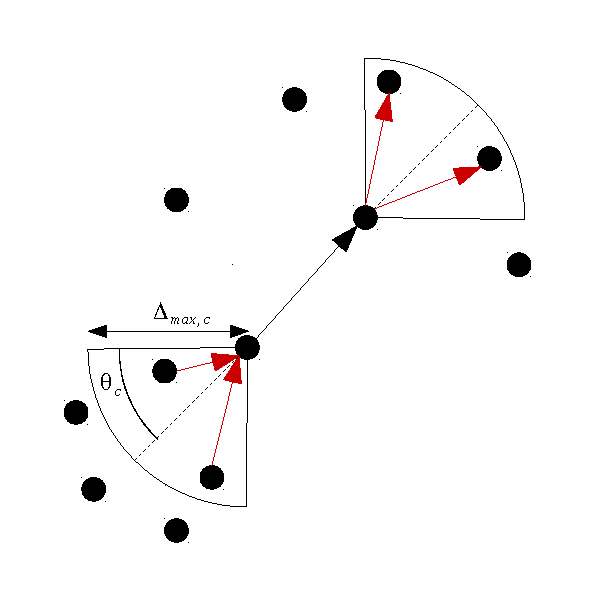
\includegraphics[width=0.8\linewidth]{ConnectorAlignment.pdf}
    \end{center}
  \end{minipage}
  \begin{minipage}{0.58\linewidth}
    \begin{center}
      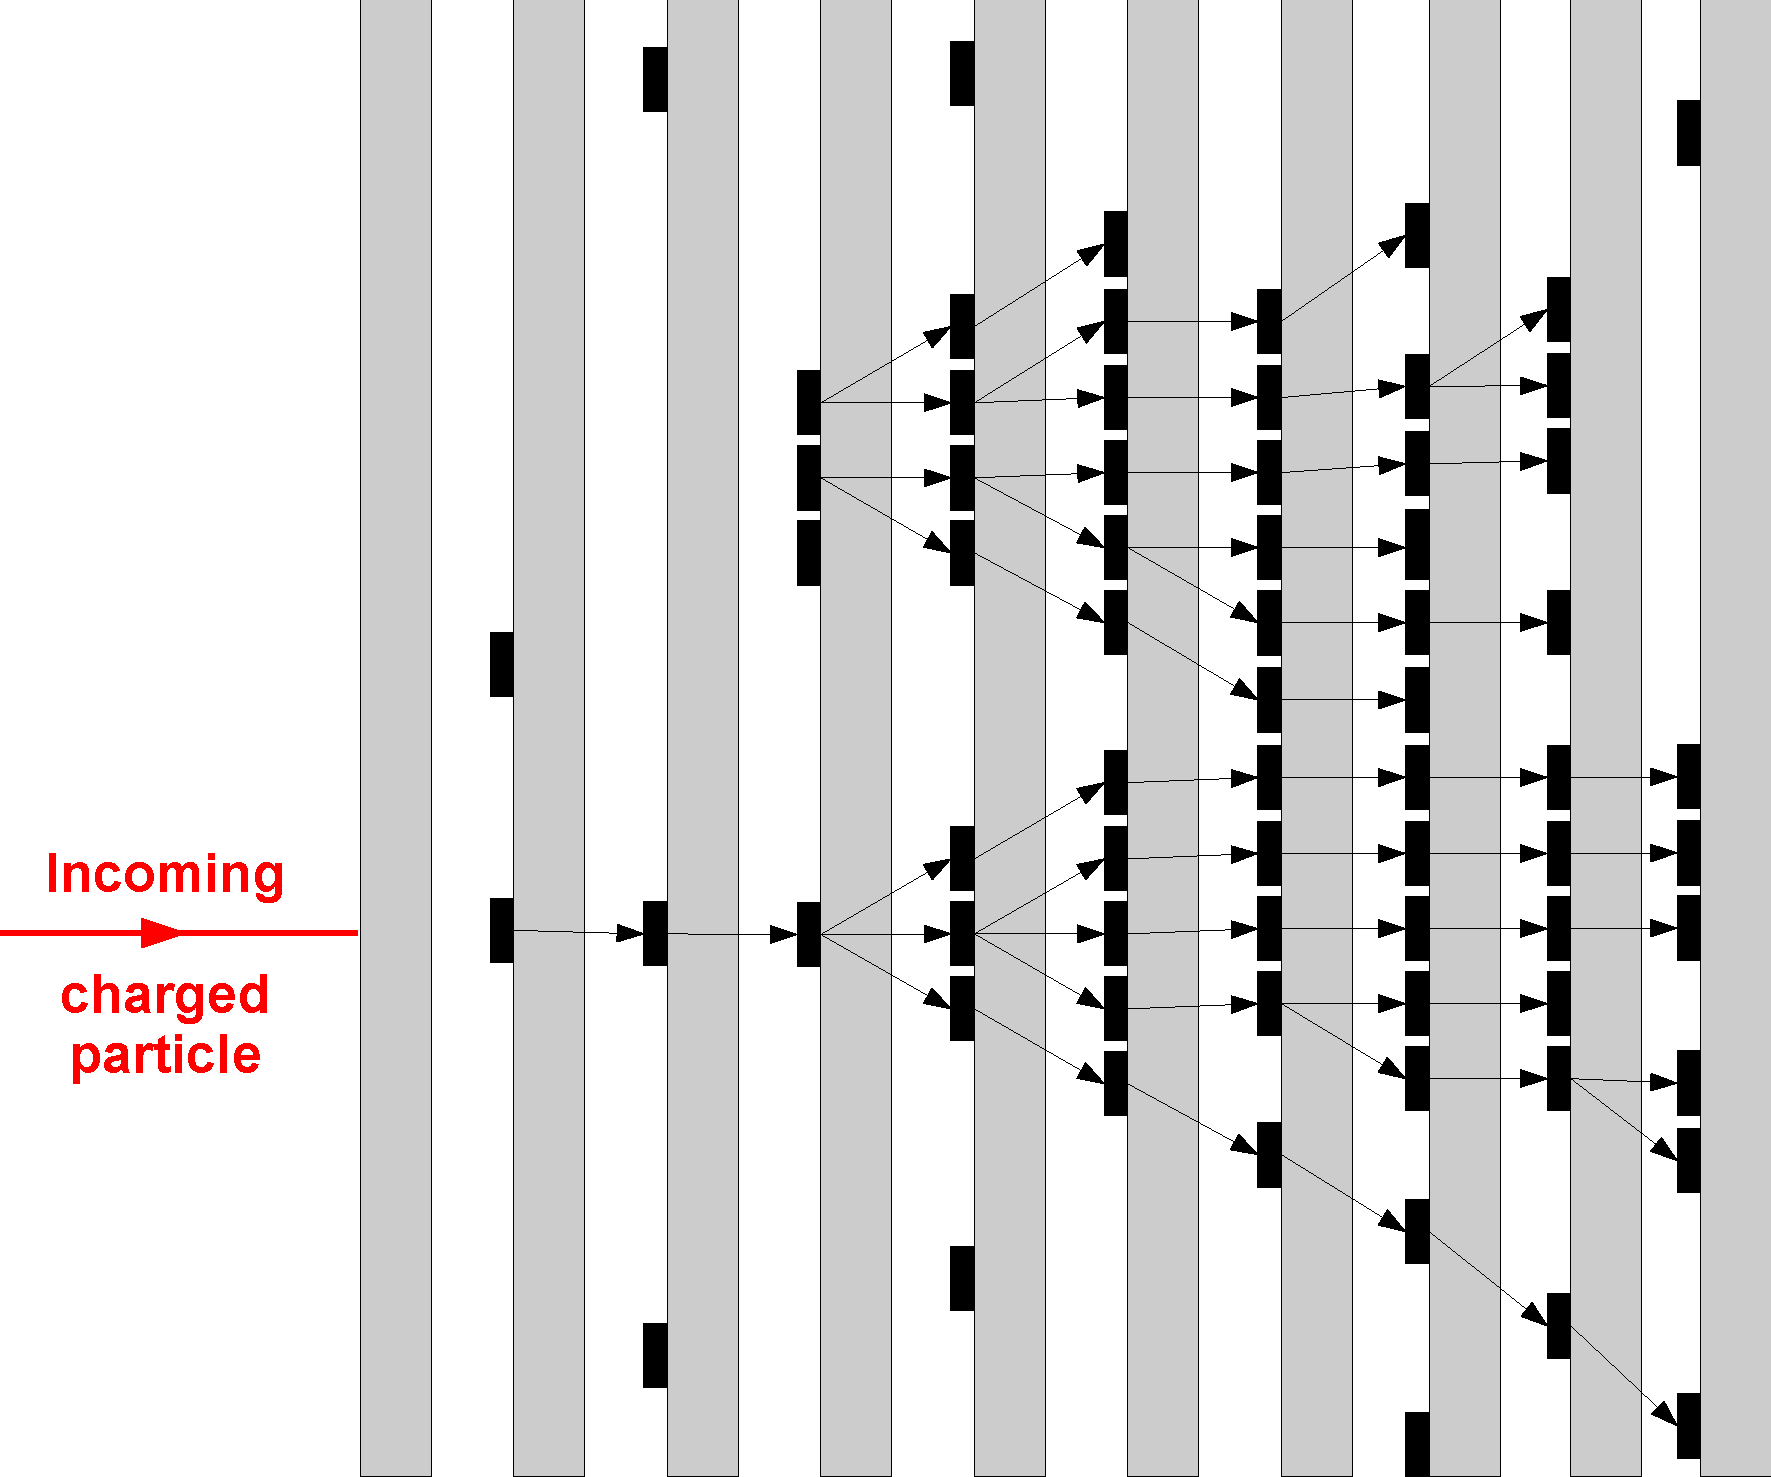
\includegraphics[width=0.8\linewidth]{ConnectorCleaning2.pdf}
    \end{center}
  \end{minipage}
  \caption{\label{ARBOR_CONNECTOR_ALIGNEMENT} \label{ARBOR_CONNECTOR_CLEANING_2} Left : Schematic view of the connector alignment procedure. In black, a considered connector and in red possible new connectors in backward and forward directions. Right : a neutral and a charged pion showers after the second connector cleaning algorithm}
\end{figure}

\paragraph*{Connector seeding 2} This second step of connector seeding starts from the tree structure obtained after the first connector cleaning algorithm. The goal of this second step is to create an alignment of connectors within the shower. For each connector, more forward connectors are created from the forward object of this connector by looking in a cone of half-angle $\theta_c$ and a maximum distance of $\Delta_{max,c}$. In the same way, additional backward connectors are created from the backward object of this connector. A schematic view of this step is shown in figure \ref{ARBOR_CONNECTOR_ALIGNEMENT}.

\paragraph*{Connector cleaning 2} Here, we again need to clean up the backward connector list to end up with only one connector per object. This last algorithm is similar to the first connector cleaning except that the cleaning is done layer per layer starting from the downstream layers with a depth parameter $\delta$ strictly higher than one. For a given connector, this accentuates the alignment with the forward ones. We end up then with a tree structure again.

\paragraph*{Tree building} This step is straight-forward. Seed objects are identified and trees are built by recursively following the forward connected objects.

The following algorithms associate some of the trees with each other.

%%%%%%%%% ASSOCIATION ALGORITHMS %%%%%%%%%%%
\subsection*{Association algorithms}

\paragraph*{Energy driven track cluster association} The track to cluster association is performed using three different pieces of information, the cluster energy, the track momentum and the cluster topology. We first look at the track projection on the calorimeter front face. Two different cases may occur :

\begin{itemize}
  \item the particle has interacted before the calorimeter or in the first layer. In this case, many seed objects are found in the N$_{layer}$ first layers at a maximum distance of $\Delta_{{track-cluster}_1}$ of the track projection. Seed objects are then sorted by their distance to the track projection. The clusters associated to their seeds are then associated to the track progressively starting from the closest one until the difference between the track momentum and the total cluster energy is minimized. The clusters are then merged since they belong to the same cluster structure.
  \item the particle produced a track segment at least in the N$_{layer}$ first layers and a seed object is found within a distance $\Delta_{(track-cluster)_1}$ to the track projection. Since only a cluster starting with a track segment has to be associated, an additional distance cut $\Delta_{(track-cluster)_2}$ between seed objects and the track projection is applied. This decreases the confusion for small separation distances between nearby particles. The same track-to-cluster association and cluster merging is then performed as above.
\end{itemize}

\begin{minipage}{0.58\linewidth}
  \vspace{-2ex}
  \begin{center}
    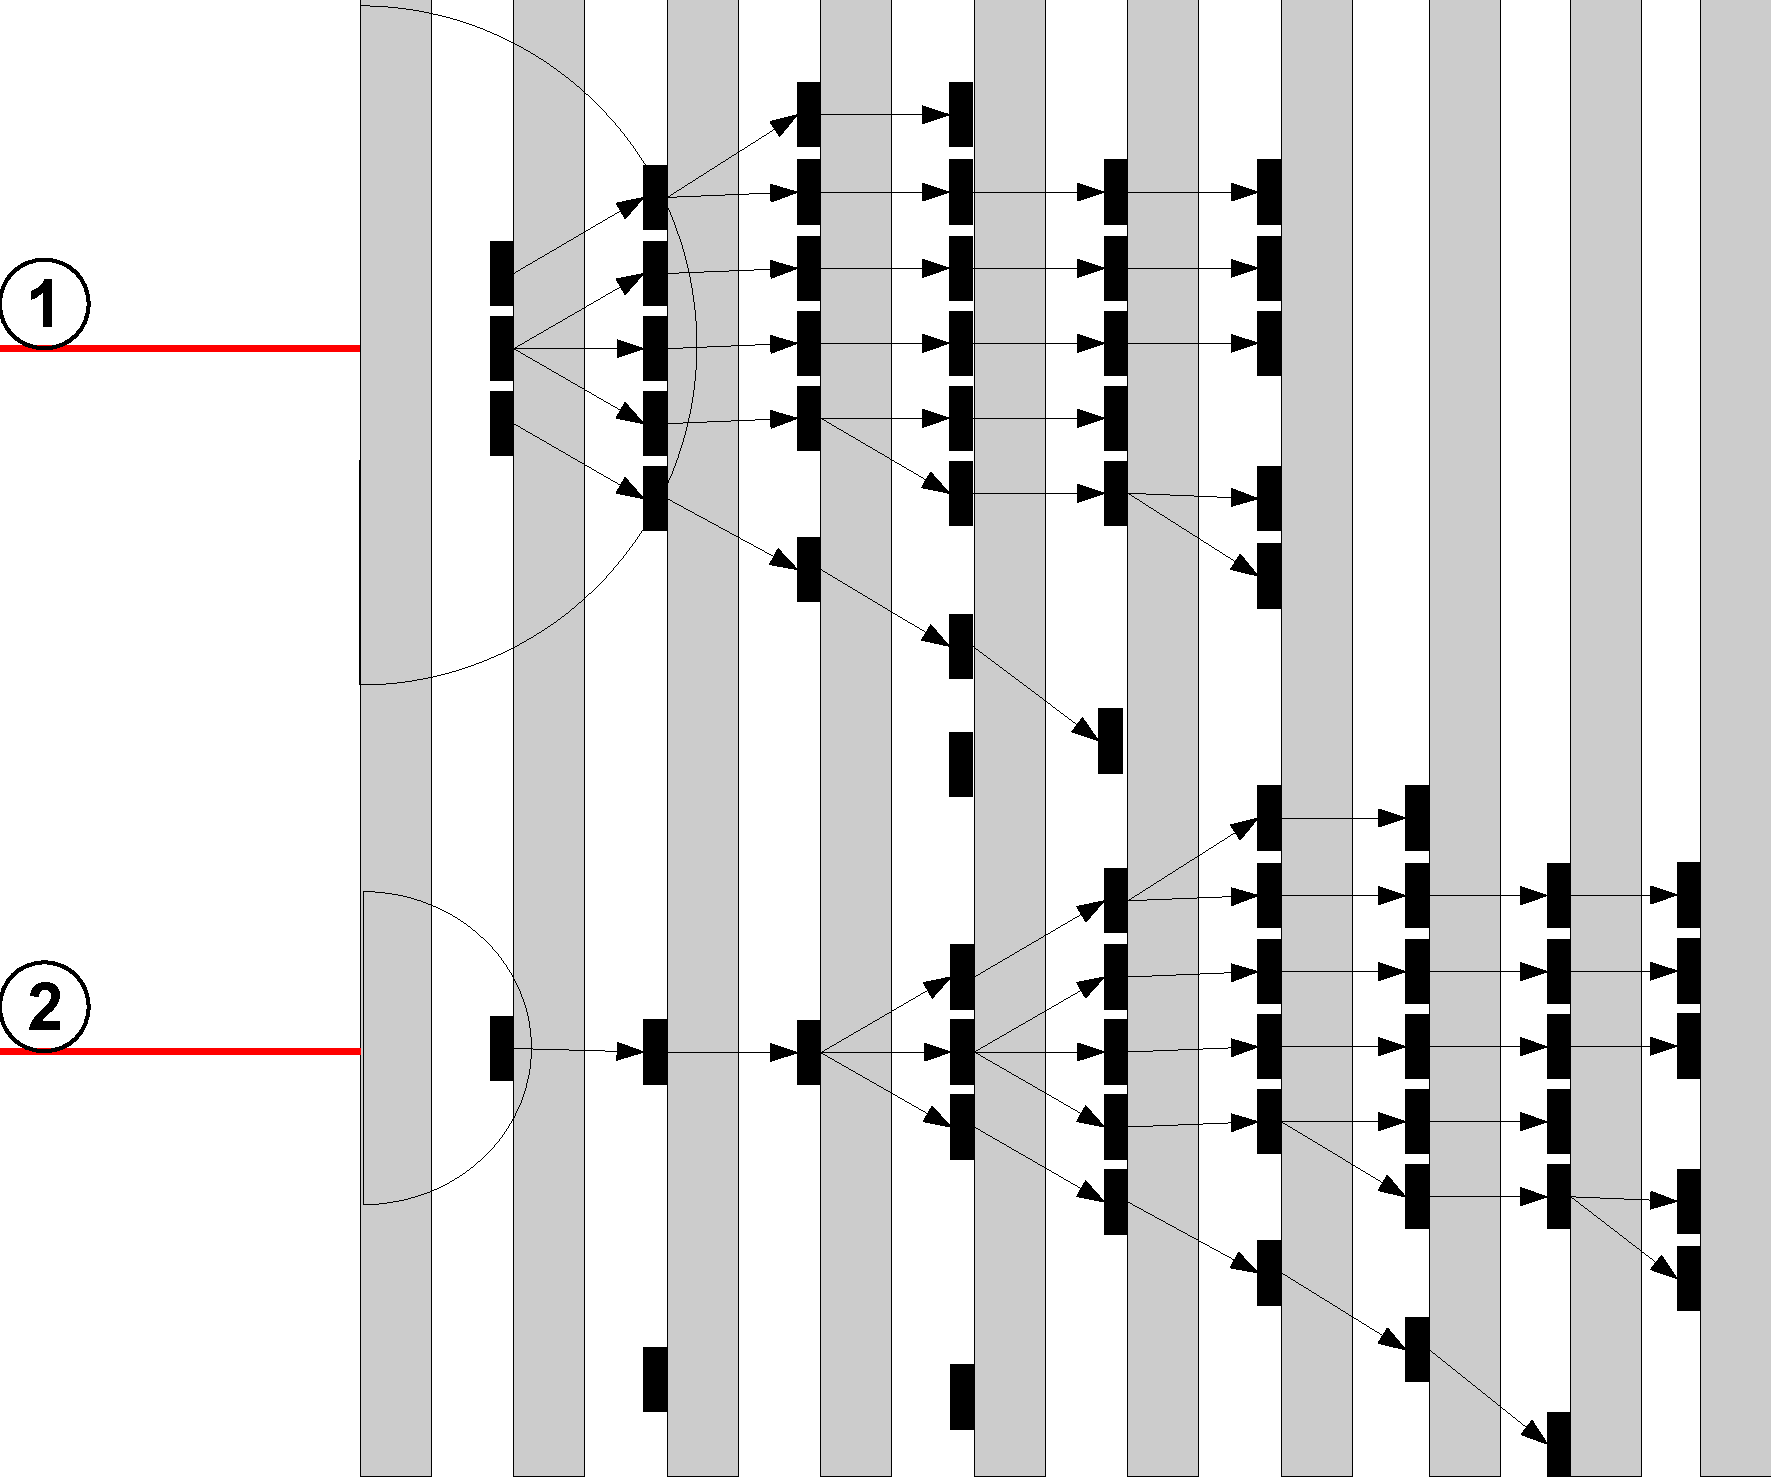
\includegraphics[width=0.7\linewidth]{EnergyDrivenTrackClusterAssociation.pdf}
    \captionof{figure}{\label{ARBOR_ENERGY_DRIVEN_TRACK_CLUSTER_ASSOCIATION} Schematic view of the energy driven track cluster algorithm.}
  \end{center}
\end{minipage}
\begin{minipage}{0.4\linewidth}
  \vspace{-2ex}
  \begin{center}
    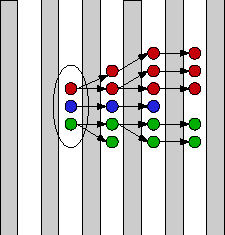
\includegraphics[width=0.8\linewidth]{NeutralTreeMerging.pdf}
    \captionof{figure}{\label{ARBOR_NEUTRAL_TREE_MERGING} Schematic view of the neutral tree merging algorithm.}
  \end{center}
\end{minipage}
\newline

Figure \ref{ARBOR_ENERGY_DRIVEN_TRACK_CLUSTER_ASSOCIATION} shows a schematic view of the two different scenarios. The upper one corresponds to the case where an early interaction is found, and the lower one where a primary track segment of a cluster is found.

\paragraph*{Neutral tree merging} This algorithm is designed for neutral particle interactions for which the first interacting layer contains a few seeds. Figure \ref{ARBOR_NEUTRAL_TREE_MERGING} shows a configuration in which three trees have been built (with three colours) for one neutral particle interaction. We can see that the seeds in the first interacting layer all belong to the same cluster. The trees having seeds closer than $\Delta_{seed}$ and positioned in the same layer are merged.

\paragraph*{Pointing cluster association} This step aims at associating neutral fragments (daughter cluster) to other fragments which may be charged or neutral clusters (parent clusters). We start by identifying the clusters that have at least N$_{objects}$ objects in at least N$_{layer}$ contiguous layers. The selected cluster could be either a parent or a daughter cluster. Then we proceed as follows :

\begin{enumerate}
  \item A linear 3D straight line fit is performed over the position of all the hits of each cluster (without weights). This defines the axis of each cluster.
  \item The clusters are sorted by their most downstream layers (most downstream hit in the cluster) l$_{inner}$.
  \item Starting from the most downstream cluster \textit{i}, we look for a parent cluster \textit{j} for which it propagates further downstream (l$_{inner,i}$~>~l$_{inner,j}$)
  \item Among these candidate parent clusters, we look for those for which d$_{proj}$ < d$_{proj,cut}$ and $\theta_{i,j}$ < $\theta_{i,j,cut}$  where :
  \begin{itemize}
    \item d$_{proj}$ is the distance between the candidate daughter cluster axis and the candidate parent cluster barycentre (line-to-point distance)
    \item $\theta_{i,j}$ is the angle between the axis of the two clusters
  \end{itemize}
  and we choose the cluster for which d$_{proj}$ is minimal.  
  \item Among this same list of candidate parent clusters, we look for those satisfying the condition d$_{cross}$ < d$_{cross,cut}$ and d$_{closest}$ < d$_{closest,cut}$ where :
  \begin{itemize}
    \item d$_{cross}$ is the distance at closest approach (d.c.a) between the two cluster axes
    \item d$_{closest,i,j}$ is the closest distance between an object of the parent cluster and the point of closest approach of the cluster axes (distance at closest approach)
  \end{itemize}
  and we choose the cluster for which d$_{cross}$ is minimal.
  \item We choose the best candidate parent cluster among the two previous methods above. Many cases may happen i) no parent cluster is found, then no parent cluster is assigned to this daughter cluster, ii) one of the two methods has found a parent cluster or the two methods provide the same parent, then we assign it to the daughter cluster, iii) the two methods have found a parent cluster but there are not the same one. In this case the closest candidate parent cluster among the two in terms of barycentre distance is assigned to the daughter cluster.
  \item If no parent cluster has been found for a cluster, nothing is done.
  \item If the parent cluster has no associated track, merge the two clusters, otherwise we define the variable $\Psi$ as :
  \begin{equation}
    \label{PSI2_ALGORITHM_EQUATION}
    \Psi = \Big| \frac{p-E_{tot}}{f_{res} . \sigma_E . p} \Big|
  \end{equation}
  where :
  \begin{itemize}
    \item p is the track momentum of the parent cluster
    \item E$_{tot}$ is the total energy estimated from the combined hit list of the parent and daughter clusters
    \item $\sigma_E$ is the calorimeter energy resolution at the track momentum p
    \item f$_{res}$ is a multiplicative factor\footnote{The parameter f$_{res}$ is used to reduce or enlarge the accepted range of the difference p-E$_{tot}$. A higher value of this parameter will accept a merging with a higher difference p-E$_{tot}$.}
  \end{itemize}
  
\begin{figure}[!h]
  \begin{center}
    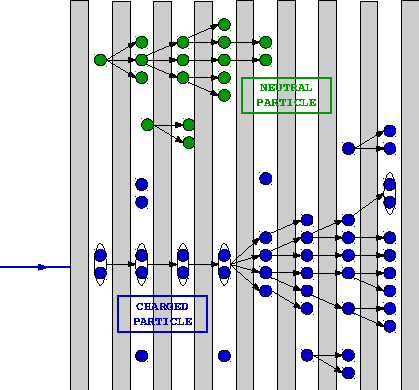
\includegraphics[width=0.4\linewidth]{PfoCreation.pdf}
  \end{center}
  \caption{\label{ARBOR_PFO_CREATION} Schematic view of the final ArborPFA output}
\end{figure}

We check then that the $\Psi$ defined for the parent and daughter clusters is less than $\Psi_{cut}$ and if the difference between p and E$_{tot}$ after the cluster merging (parent + daughter clusters) decreases. The two clusters are merged if the previous conditions are satisfied.

\end{enumerate}

\paragraph*{Small neutral fragment merging} At this stage, the main part of the shower of each particles has been identified. Only isolated objects and small tree structures that surround the showers are not associated. First, these small structures are identified if their size is less than $N_{cut}$ objects. Then every small structure is merged within a shower, the closest in terms of barycentre distances.

\paragraph*{Particle flow object creation} Particle flow objects are built from the produced clusters after all the steps described above (Figure \ref{ARBOR_PFO_CREATION}). Charged PFOs are built from clusters that have an associated track, while other clusters are considered as neutral PFOs.

\newpage
\section{ArborPFA algorithm parameters}
\label{ARBOR_ALGORITHM_PARAMETERS}

% Object creation
\paragraph{Object creation algorithm} ~

\begin{table}[!h]
  \begin{center}
    \begin{tabu} to \linewidth { c | c } 
          Parameter name & value \\
          \hline
          MaxClusterSize & 4 \\
          IntraLayerDistance & 11 mm
    \end{tabu} 
  \end{center}
\end{table}

\begin{itemize}
 \item MaxClusterSize \\
 $\rightarrow$ The maximum intra layer cluster size to build an object with. Else the object is split in single calo hit objects
 \item IntraLayerDistance \\
 $\rightarrow$ The nearest neighbour intra layer clustering maximum distance
\end{itemize}


% Track segment candidate tagging
\paragraph{Track segment candidate tagging algorithm} ~

\begin{table}[!h]
  \begin{center}
    \begin{tabu} to \linewidth { c | c } 
          Parameter name & value \\
          \hline
          MaxNNeighbors & 6 \\
          IntraLayerNeighbourDistance ($\Delta_{mip}$) & 50 mm
    \end{tabu} 
  \end{center}
\end{table}

\begin{itemize}
  \item MaxNNeighbors \\
  $\rightarrow$ The maximum number of neighbouring objects within a layer
  \item IntraLayerNeighbourDistance ($\Delta_{mip}$) \\
  $\rightarrow$ The maximum distance between two neighbours in a layer used for the neighbour counting
\end{itemize}

\newpage
% Primary track connection
\paragraph{Primary track connection} ~

\begin{table}[!ht]
  \begin{center}
    \begin{tabu} to \linewidth { c | c } 
          Parameter name & value \\
          \hline
          ConnectionDistance & 110 mm \\ 
          BackwardConnectorWeight & 2 \\ 
          ForwardConnectorWeight & 3 \\ 
          OrderParameterAnglePower & 1 \\ 
          OrderParameterDistancePower & 5 \\
          MaxNEmptyConsecutiveLayers & 3 
    \end{tabu} 
  \end{center}
\end{table}

\begin{itemize}
  \item ConnectionDistance \\
  $\rightarrow$ The maximum connection distance used for the primary track connectors creation
  \item BackwardConnectorWeight ($w_{bck}$) \\
  $\rightarrow$ The backward connector weight assigned for the reference vector computation
  \item ForwardConnectorWeight ($w_{fwd}$) \\
  $\rightarrow$ The forward connector weight assigned for the reference vector computation
  \item OrderParameterAnglePower \\ 
  $\rightarrow$ The angle power parameter of the $\kappa$ parameter while cleaning connectors
  \item OrderParameterDistancePower \\
  $\rightarrow$ The distance power parameter of the $\kappa$ parameter while cleaning connectors
  \item MaxNEmptyConsecutiveLayers \\
  $\rightarrow$ The maximum consecutive empty layers to take into account for the connector seeding
\end{itemize}


% Connector seeding 1
\paragraph{Connector seeding 1} ~

\begin{table}[!ht]
  \begin{center}
    \begin{tabu} to \linewidth { c | c } 
          Parameter name & value \\
          \hline
          ConnectionDistance & 45 mm
    \end{tabu} 
  \end{center}
\end{table}

\begin{itemize}
  \item ConnectionDistance \\
  $\rightarrow$ The maximum connection distance used for a connector creation
\end{itemize}


\newpage
% Connector cleaning 1
\paragraph{Connector cleaning 1} ~

\begin{table}[!ht]
  \begin{center}
    \begin{tabu} to \linewidth { c | c } 
          Parameter name & value \\
          \hline
          BackwardConnectorWeight & 2 \\
          ForwardConnectorWeight & 2 \\
          OrderParameterAnglePower & 1 \\
          OrderParameterDistancePower & 5 \\
          ReferenceDirectionDepth & 1
    \end{tabu} 
  \end{center}
\end{table}

\begin{itemize}
  \item BackwardConnectorWeight \\
  $\rightarrow$ The weight of a backward connector assigned in the reference direction vector calculation.
  \item ForwardConnectorWeight \\
  $\rightarrow$ The weight of a forward connector assigned in the reference direction vector calculation.
  \item OrderParameterAnglePower \\
  $\rightarrow$ The $\theta$ angle power parameter used for the $\kappa$ parameter computation
  \item OrderParameterDistancePower \\
  $\rightarrow$ The $\Delta$ distance power parameter used for the $\kappa$ parameter computation
  \item ReferenceDirectionDepth \\
  $\rightarrow$ The forward connector depth used for the reference vector computation
\end{itemize}


% Connector seeding 2
\paragraph{Connector seeding 2} ~

\begin{table}[!ht]
  \begin{center}
    \begin{tabu} to \linewidth { c | c } 
          Parameter name & value \\
          \hline
          ConnectionDistance & 65 mm \\
          ConnectionAngle & 0.7 rad
    \end{tabu} 
  \end{center}
\end{table}

\begin{itemize}
  \item ConnectionDistance \\
  $\rightarrow$ The maximum connection distance used for a connector creation
  \item ConnectionAngle \\
  $\rightarrow$ The maximum angle between two connectors
\end{itemize}


\newpage
% Connector cleaning 2
\paragraph{Connector cleaning 2} ~

\begin{table}[!ht]
  \begin{center}
    \begin{tabu} to \linewidth { c | c } 
          Parameter name & value \\
          \hline
          BackwardConnectorWeight & 0.1 \\
          ForwardConnectorWeight & 5 \\
          OrderParameterAnglePower & 1 \\
          OrderParameterDistancePower & 5 \\
          ReferenceDirectionDepth & 2
    \end{tabu} 
  \end{center}
\end{table}

\begin{itemize}
  \item BackwardConnectorWeight \\
  $\rightarrow$ The weight of a backward connector assigned in the reference direction vector calculation.
  \item ForwardConnectorWeight \\
  $\rightarrow$ The weight of a forward connector assigned in the reference direction vector calculation.
  \item OrderParameterAnglePower \\
  $\rightarrow$ The $\theta$ angle power parameter used for the $\kappa$ parameter computation
  \item OrderParameterDistancePower \\
  $\rightarrow$ The $\Delta$ distance power parameter used for the $\kappa$ parameter computation
  \item ReferenceDirectionDepth \\
  $\rightarrow$ The forward connector depth used for the reference vector computation
\end{itemize}


% Energy driven track cluster association
\paragraph{Energy driven track cluster association} ~

\begin{table}[!ht]
  \begin{center}
    \begin{tabu} to \linewidth { c | c } 
          Parameter name & value \\
          \hline
          TrackToClusterDistanceCut1 & 75 mm \\
          TrackToClusterDistanceCut2 & 55 mm \\
          FirstInteractingLayerNSeedCut & 15 \\
          TrackToClusterNLayersCut & 3 \\
          TrackClusterPsi2Cut & 3 \\
          Psi2SigmaFactor & 1.5
    \end{tabu} 
  \end{center}
\end{table}

\begin{itemize}
  \item TrackToClusterDistanceCut1 \\
  $\rightarrow$ The maximum distance between the track projection at calorimeter front face and a cluster seed. This distance is used to detect an early interacting cluster.
  \item TrackToClusterDistanceCut2 \\
  $\rightarrow$ The reduced maximum distance between the track projection at calorimeter front face and a cluster seed. This distance is used when no early interacting cluster has been detected.
  \item FirstInteractingLayerNSeedCut \\
  $\rightarrow$ The cut on the number of cluster seeds found within a the distance TrackToClusterDistanceCut1 to detect an early cluster interaction.
  \item TrackToClusterNLayersCut \\
  $\rightarrow$ The number of inner layers to look for cluster seeds to associate.
  \item TrackClusterPsi2Cut \\
  $\rightarrow$ The $\psi^2$ cut applied while associating clusters to a track.
  \item Psi2SigmaFactor \\
  $\rightarrow$ The $f_{res}$ factor on denominator used to compute the $\psi^2$ for track-to-cluster compatibility (see equation \ref{PSI2_ALGORITHM_EQUATION})
\end{itemize}


% Neutral tree merging
\paragraph{Neutral tree merging} ~

\begin{table}[!ht]
  \begin{center}
    \begin{tabu} to \linewidth { c | c } 
          Parameter name & value \\
          \hline
          SeedSeparationMerge ($\Delta_{seed}$) & 25 mm
    \end{tabu}
  \end{center}
\end{table}

\begin{itemize}
  \item SeedSeparationMerge ($\Delta_{seed}$) \\
  $\rightarrow$ The maximum distance between two cluster seeds within a layer to perform a cluster merging
\end{itemize}


% Pointing cluster association
\paragraph{Pointing cluster association} ~

\begin{table}[!ht]
  \begin{center}
    \begin{tabu} to \linewidth { c | c } 
          Parameter name & value \\
          \hline
          MinNObjects & 4 \\
          MinNLayers & 4 \\
          FitToBarycentreDistanceCut & 30 mm \\
          FitToBarycentreAngleCut & $\frac{\pi}{6}$ rad \\
          FitToFitDistanceCut & 20 mm \\
          FitDistanceApproachCut & 20 mm \\
          Chi2NSigmaFactor & 1.5 \\
          Chi2AssociationCut & 1
    \end{tabu}
  \end{center}
\end{table}

\begin{itemize}
  \item MinNObjects \\
  $\rightarrow$ The minimum number of objects within a cluster in order to to be candidate for the pointing cluster association
  \item MinNLayers \\
  $\rightarrow$ The minimum number of layers within a cluster (outermost - innermost + 1) in order to be candidate for the pointing cluster association
  \item FitToBarycentreDistanceCut \\
  $\rightarrow$ The cut applied on the distance between the daughter cluster fit and the parent cluster barycentre position (point-to-line distance)
  \item FitToBarycentreAngleCut \\
  $\rightarrow$ The cut applied on the angle between the daughter and parent cluster fits
  \item FitToFitDistanceCut \\
  $\rightarrow$ The cut applied on the distance between the daughter and parent cluster fits (line-to-line distance)
  \item FitDistanceApproachCut \\
  $\rightarrow$ The cut applied on the closest distance between a parent cluster object and the daughter cluster crossing point at the parent and daughter cluster fit closest approach.
  \item Chi2NSigmaFactor \\
  $\rightarrow$ The $N_{res}$ factor on denominator used to compute the $\chi^2$ for track-to-cluster compatibility (see equation \ref{PSI2_ALGORITHM_EQUATION}) using the merged cluster (daughter + parent)
  \item Chi2AssociationCut \\
  $\rightarrow$ The $\chi^2$ cut applied on the merged clusters compatibility with a track when associating a neutral daughter cluster with a charged parent cluster.
\end{itemize}


% Small neutral fragment merging
\paragraph{Small neutral fragment merging} ~

\begin{table}[!ht]
  \begin{center}
    \begin{tabu} to \linewidth { c | c } 
          Parameter name & value \\
          \hline
          MaximumDaughterNObject & 20 \\
          LargeDistanceCut & 1000 mm
    \end{tabu}
  \end{center}
\end{table}

\begin{itemize}
  \item MaximumDaughterNObject \\
  $\rightarrow$ The maximum number of objects to consider the cluster as a small neutral fragment to merge it into a bigger parent cluster
  \item LargeDistanceCut \\
  $\rightarrow$ The maximum distance between a small neutral fragment and a potential parent cluster
\end{itemize}

\end{document}
